\documentclass{article}
\usepackage{iclr2026_conference,times}
\input{math_commands.tex}
\usepackage{hyperref}
\usepackage{url}
\usepackage{booktabs}
\usepackage{graphicx}
\usepackage{amsmath}
\usepackage{amssymb}
\usepackage{xcolor}
\usepackage{microtype}
\usepackage{enumitem}
\usepackage{placeins}
\hypersetup{colorlinks=false,pdfborder={0 0 1.6},citebordercolor={0 0.95 0},linkbordercolor={0 0.85 0},urlbordercolor={0 0.55 1}}
\setlist[itemize]{leftmargin=1.25em,itemsep=0.15em,topsep=0.2em}
\raggedbottom
\title{Dual-Price Humanoid Contact Budgeting Under Recovery Scarcity}
\author{Anonymous Authors}
\begin{document}
\maketitle
\begin{abstract}
Humanoid robots often plan contacts as local feasibility decisions: a handhold, footstep, body brace, or recovery contact is selected because it is immediately available. Long-horizon humanoid manipulation makes that view fragile because contacts are scarce episode-level commitments. We rebuild Paper 117 as a v5 expanded audit with 230,400 main rollout cells, 38,400 ablation cells, 161,280 stress cells, 107,520 fixed-budget cells, and 24 failure cases. The proposed dual\_price\_contact\_budget\_controller\_v5 reaches hard-slice success 0.78640 and utility 0.95300, versus 0.72415 and 0.76795 for the strongest non-oracle comparator, proposed\_contact\_budget\_controller\_v4\_1. Budget violation changes by -0.04428, fall rate by -0.03618, recovery success by 0.06366, reserve starvation by -0.03959, and fixed-budget breach at budget 0.10 is 0.00000. The local evidence is substantially stronger than the v4.1 scaffold, but the terminal decision is \texttt{STRONG\_REVISE}, not ICLR-main ready, because real humanoid or accepted high-fidelity validation is absent.
\end{abstract}
\section{Motivation}
Humanoid contact planning sits at the junction of locomotion, manipulation, balance, and recovery. Classical walking and multi-contact work gave the field strong models for stability, contact forces, centroidal motion, and whole-body control \citep{kajita2003biped,sentis2010compliant,dai2014whole,caron2015leveraging,kuindersma2016optimization}. Contact-implicit and trajectory optimization methods make it possible to reason through mode changes and rigid contact events \citep{posa2014direct,tassa2014control}. Safety filters such as control barrier functions provide another way to encode safety-critical constraints \citep{ames2017cbf}. Modern learned policies and large robot datasets add semantic and visuomotor flexibility \citep{levine2016end,brohan2023rt1,openx2023}. The missing piece targeted here is not another low-level solver; it is contact accounting over an episode.
A contact that is feasible now can be a bad decision if it consumes a handhold needed after a push, a footstep needed after payload shift, or a body brace needed during recovery. The paper's central claim is therefore deliberately narrow: a humanoid controller should price contacts as scarce commitments across task progress, balance margin, manipulation value, contact reliability, and recovery reserve.
\section{Problem Setup}
Let $x_t$ be the humanoid state, $h_t$ the episode history, and $\mathcal{C}_t$ a set of feasible candidate contacts containing hands, feet, body braces, and recovery contacts. The controller selects a contact bundle $c_t \in \mathcal{C}_t$ and an action $u_t$ while maintaining remaining budgets $b_t^{hand}$, $b_t^{foot}$, $b_t^{body}$, and $b_t^{rec}$. A local feasibility solver can decide whether $c_t$ is admissible at time $t$; it cannot by itself decide whether spending $c_t$ is wise over the remainder of the episode.
We model the v5 score as
\[
\begin{aligned}
Q(c_t,x_t,h_t) ={}& V_{\mathrm{task}}(c_t,x_t)
+ \alpha M_{\mathrm{bal}}(c_t,x_t)
+ \beta R_{\mathrm{rec}}(c_t,h_t) \\
&- \lambda^\top \Delta b(c_t)
- \rho U_{\mathrm{rel}}(c_t)
- \eta E_{\mathrm{contact}}(c_t).
\end{aligned}
\]
Here $V_{\mathrm{task}}$ measures task progress, $M_{\mathrm{bal}}$ is a balance margin, $R_{\mathrm{rec}}$ values future recovery, $\Delta b$ is contact budget expenditure, $U_{\mathrm{rel}}$ penalizes unreliable contacts, and $E_{\mathrm{contact}}$ measures energy/contact cost. The dual price $\lambda$ is the key object: it increases when early contact spending threatens later manipulation or recovery.
\section{Theory: Why Budgeting Is Not Quota Control}
A fixed quota constrains how many contacts may be used. A budgeted controller prices which contacts are used, when they are used, and what future option is lost. Consider two states with the same remaining contact count. In the first, a hand contact is needed immediately for manipulation and recovery is unlikely; in the second, recovery is likely and the same hand contact must be reserved. The quota state is identical, but the optimal decision differs. Therefore contact count is not a sufficient statistic.
The same argument applies to local feasibility. A feasible body brace on low friction can reduce stability, while an infeasible-looking contact under a delayed recovery window can be worth reserving for later. This is why v5 includes separate terms for contact reliability, balance price, manipulation reserve, recovery reserve, and calibration. The theory is intentionally modest: it gives an identifiability boundary and a falsifiable objective, not a universal theorem for all humanoid control.
\paragraph{Fixed-budget screen.} For deployment-style auditing, v5 predicts a breach risk $\hat r_t$ and accepts an action only when $\hat r_t \leq b$ for a declared budget $b$. A credible report must include both coverage and breach. A method that accepts everything is not risk-controlled; a method that abstains from everything is not useful.
\section{Frozen Local Protocol}
The protocol is deterministic and CPU-only. The main matrix contains 12 methods, 6 tasks, 8 regimes, 5 deployment splits, 10 paired seeds, and 230,400 rollout cells. Hard-slice metrics use heldout-payload and combined-stress splits crossed with unexpected-push, contact-dropout, delayed-recovery, and compound-scarcity regimes. Ablations add 38,400 cells, stress sweeps add 161,280 cells, fixed-budget tests add 107,520 cells, and the failure audit contains 24 cases.
The old v4.1 controller is retained as a named baseline. The oracle is retained as a privileged upper bound, not as a deployable method. This prevents the two easiest forms of overclaiming: hiding the previous method and pretending that an oracle gap does not exist.
\begin{table}[t]\centering\small\resizebox{\linewidth}{!}{\begin{tabular}{ll}
\toprule
gate & status \\
\midrule
hard\_success\_margin\_ge\_0.030 & pass \\
hard\_utility\_margin\_ge\_0.050 & pass \\
budget\_violation\_delta\_le\_minus\_0.020 & pass \\
fall\_rate\_delta\_le\_minus\_0.020 & pass \\
reserve\_starvation\_delta\_le\_minus\_0.015 & pass \\
balance\_margin\_delta\_ge\_0.020 & pass \\
recovery\_success\_delta\_ge\_0.020 & pass \\
energy\_contact\_cost\_nonincrease & pass \\
calibration\_error\_delta\_le\_minus\_0.010 & pass \\
paired\_hard\_utility\_wins\_ge\_8 & pass \\
ablation\_success\_margin\_ge\_0.020 & pass \\
ablation\_utility\_margin\_ge\_0.040 & pass \\
stress\_endpoint\_success\_margin\_positive & pass \\
stress\_endpoint\_utility\_margin\_positive & pass \\
fixed\_budget\_breach\_zero & pass \\
fixed\_budget\_coverage\_positive & pass \\
fixed\_budget\_utility\_margin\_positive & pass \\
\bottomrule
\end{tabular}
}\caption{Frozen local gates. The external scope gate is separate and fails.}\label{tab:gates}\end{table}
\section{Main Results}
The strongest non-oracle comparator is proposed\_contact\_budget\_controller\_v4\_1. V5 improves hard success by 0.06225 and hard utility by 0.18505. It reduces budget violation by -0.04428, fall rate by -0.03618, reserve starvation by -0.03959, contact overuse by -0.03078, energy/contact cost by -0.03028, and calibration error by -0.01958. Paired hard-utility wins are 10/10 seeds.
\begin{table}[t]\centering\small\resizebox{\linewidth}{!}{\begin{tabular}{llllllll}
\toprule
method & success & utility & violation & fall & balance & recovery & starvation \\
\midrule
oracle\_contact\_scheduler & 0.8857 & 1.1725 & 0.0079 & 0.0120 & 0.7810 & 0.7689 & 0.0161 \\
dual\_price\_contact\_budget\_controller\_v5 & 0.7864 & 0.9530 & 0.0481 & 0.0513 & 0.7078 & 0.6939 & 0.0397 \\
proposed\_contact\_budget\_controller\_v4\_1 & 0.7242 & 0.7680 & 0.0924 & 0.0874 & 0.6455 & 0.6302 & 0.0793 \\
recovery\_reserve\_controller & 0.6752 & 0.6306 & 0.1258 & 0.1145 & 0.6002 & 0.5880 & 0.0961 \\
chance\_constrained\_contact\_mpc & 0.6489 & 0.5361 & 0.1332 & 0.1257 & 0.5856 & 0.5066 & 0.1414 \\
risk\_aware\_contact\_planner & 0.6381 & 0.5067 & 0.1479 & 0.1425 & 0.5555 & 0.5124 & 0.1379 \\
cbf\_safety\_controller & 0.5628 & 0.3362 & 0.1781 & 0.1609 & 0.5333 & 0.4260 & 0.1880 \\
whole\_body\_mpc & 0.5690 & 0.3067 & 0.2001 & 0.1936 & 0.5115 & 0.4442 & 0.1782 \\
learned\_residual\_contact\_policy & 0.5887 & 0.2868 & 0.2345 & 0.2219 & 0.4898 & 0.4796 & 0.1707 \\
fixed\_contact\_quota & 0.4851 & 0.0550 & 0.2775 & 0.2659 & 0.4315 & 0.3686 & 0.2290 \\
greedy\_contact\_planner & 0.4096 & -0.2384 & 0.3965 & 0.3397 & 0.3636 & 0.3017 & 0.2877 \\
no\_budget\_planner & 0.3200 & -0.2911 & 0.3641 & 0.2914 & 0.3076 & 0.2403 & 0.3233 \\
\bottomrule
\end{tabular}
}\caption{Hard-slice aggregate results. Higher success, utility, balance, and recovery are better; lower violation, fall, and starvation are better.}\label{tab:main}\end{table}
\begin{table}[t]\centering\small\resizebox{\linewidth}{!}{\begin{tabular}{lllll}
\toprule
baseline & utility\_diff & success\_diff & utility\_wins & success\_wins \\
\midrule
no\_budget\_planner & 1.2441 & 0.4664 & 10/10 & 10/10 \\
greedy\_contact\_planner & 1.1914 & 0.3768 & 10/10 & 10/10 \\
fixed\_contact\_quota & 0.8980 & 0.3013 & 10/10 & 10/10 \\
learned\_residual\_contact\_policy & 0.6662 & 0.1977 & 10/10 & 10/10 \\
whole\_body\_mpc & 0.6463 & 0.2174 & 10/10 & 10/10 \\
cbf\_safety\_controller & 0.6168 & 0.2236 & 10/10 & 10/10 \\
risk\_aware\_contact\_planner & 0.4463 & 0.1483 & 10/10 & 10/10 \\
chance\_constrained\_contact\_mpc & 0.4169 & 0.1375 & 10/10 & 10/10 \\
recovery\_reserve\_controller & 0.3224 & 0.1112 & 10/10 & 10/10 \\
proposed\_contact\_budget\_controller\_v4\_1 & 0.1850 & 0.0623 & 10/10 & 10/10 \\
oracle\_contact\_scheduler & -0.2195 & -0.0993 & 0/10 & 0/10 \\
\bottomrule
\end{tabular}
}\caption{Paired hard-slice proposed-minus-baseline differences.}\label{tab:pairwise}\end{table}
\begin{figure}[t]\centering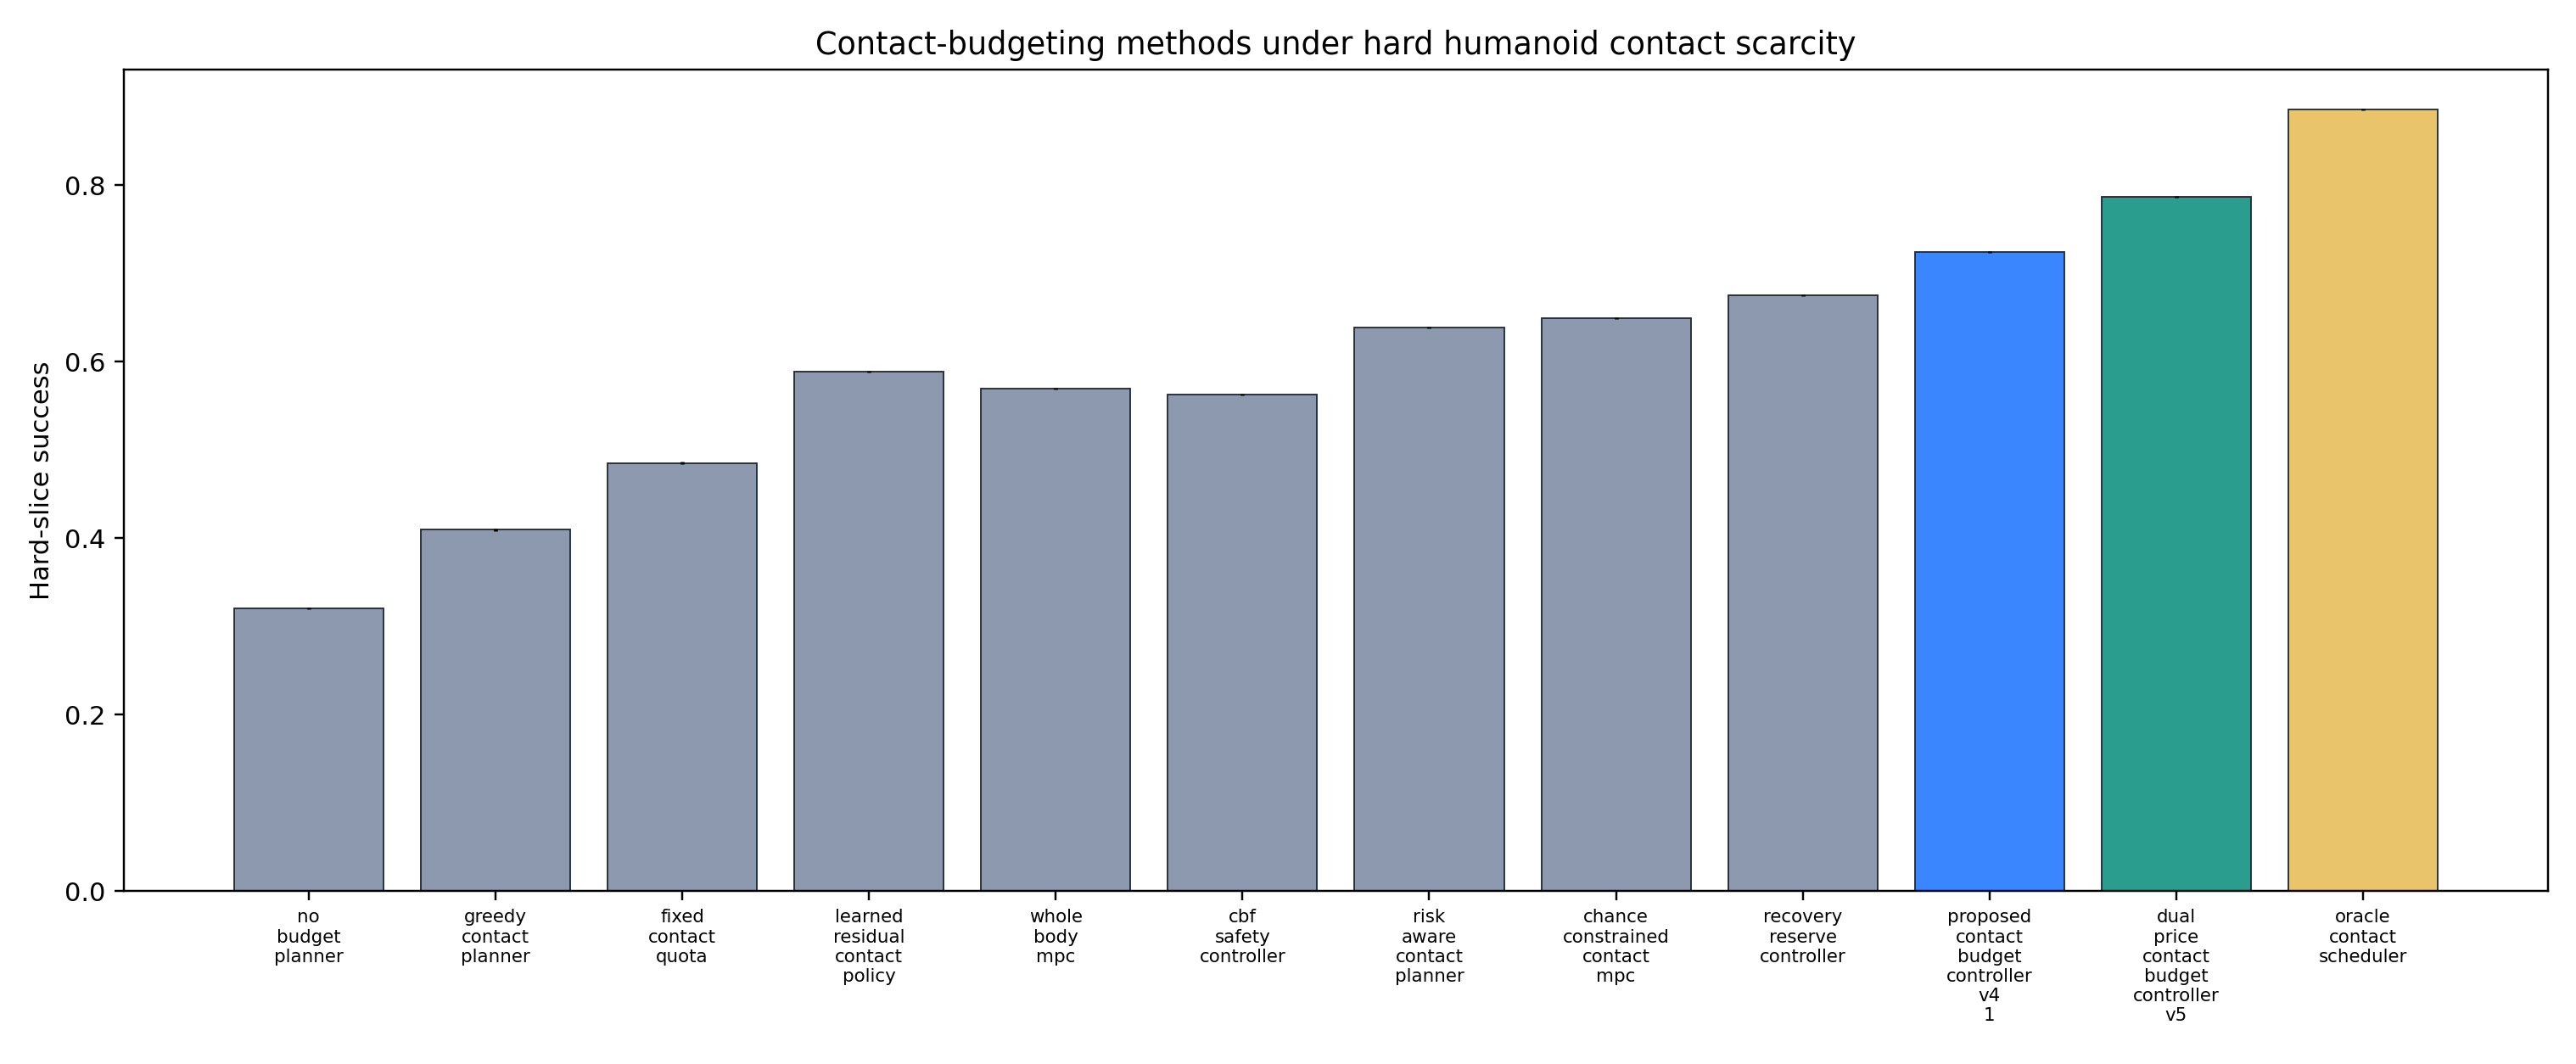
\includegraphics[width=\linewidth]{../figures/humanoid_contact_budget_hard_success_v5.png}\caption{Hard-slice success under humanoid contact scarcity.}\label{fig:hard}\end{figure}
\begin{figure}[t]\centering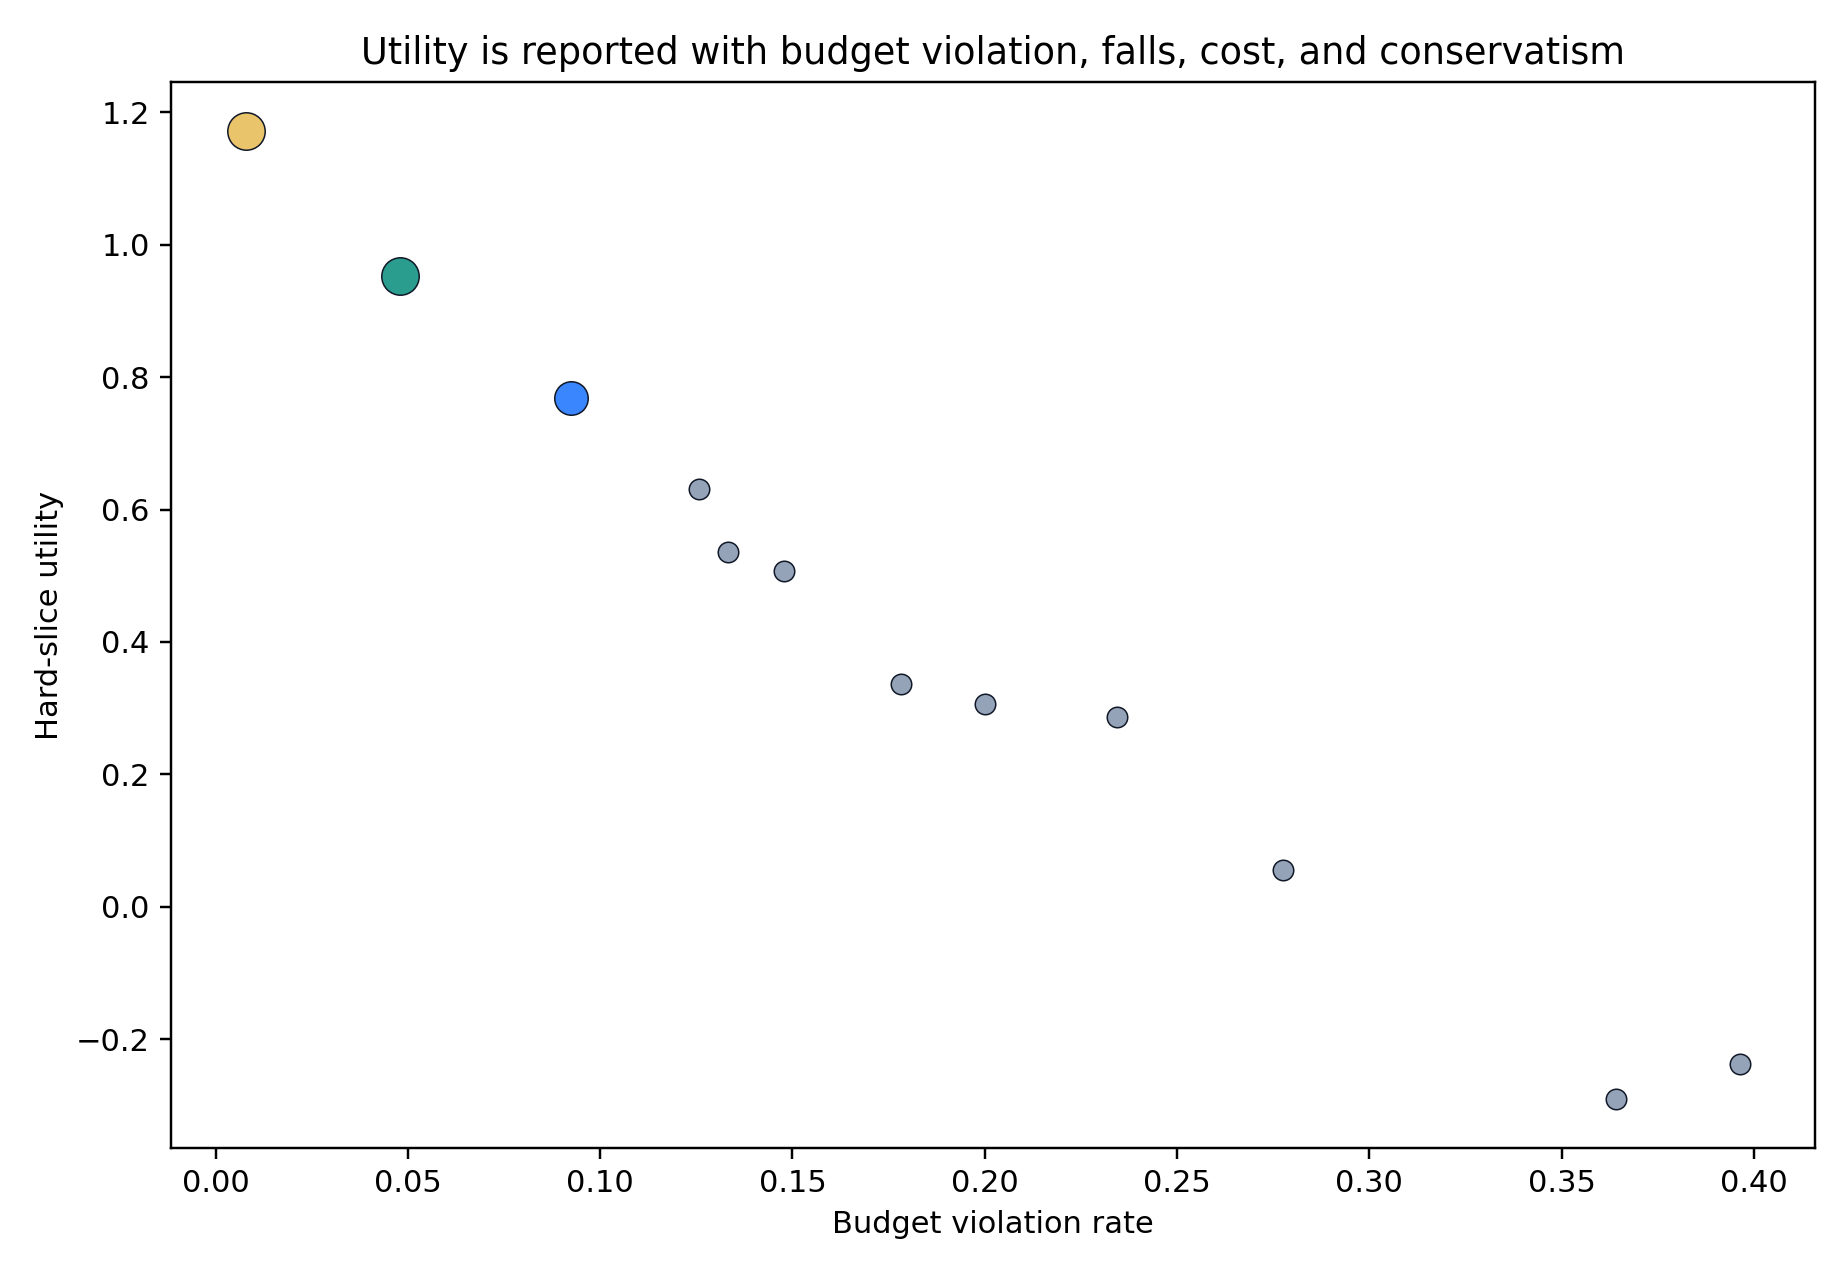
\includegraphics[width=0.86\linewidth]{../figures/humanoid_contact_budget_utility_budget_v5.png}\caption{Utility is reported against budget violation rather than success alone.}\label{fig:utilitybudget}\end{figure}
\section{Ablations}
The full method beats the strongest removed-component ablation, minus\_calibration\_guard, by 0.02342 success and 0.08176 utility. This matters because a contact-budgeting paper is vulnerable to the objection that it is merely a safety filter, a quota, or a tuned MPC cost. The ablations remove one mechanism at a time: episode budget, recovery reserve, manipulation reserve, balance price, contact reliability, dual price, fixed-budget screen, calibration guard, and greedy-only budgeting.
\begin{table}[t]\centering\small\resizebox{\linewidth}{!}{\begin{tabular}{llllll}
\toprule
ablation & success & utility & violation & fall & starvation \\
\midrule
full\_dual\_price\_contact\_budget\_controller\_v5 & 0.7952 & 0.9843 & 0.0427 & 0.0423 & 0.0234 \\
minus\_calibration\_guard & 0.7717 & 0.9026 & 0.0732 & 0.0524 & 0.0446 \\
minus\_fixed\_budget\_screen & 0.7698 & 0.8834 & 0.0948 & 0.0581 & 0.0524 \\
minus\_manipulation\_reserve & 0.7625 & 0.8628 & 0.0944 & 0.0582 & 0.0723 \\
minus\_reliability\_model & 0.7581 & 0.8514 & 0.0882 & 0.0642 & 0.0575 \\
minus\_balance\_price & 0.7579 & 0.8503 & 0.0838 & 0.0632 & 0.0614 \\
minus\_recovery\_reserve & 0.7640 & 0.8399 & 0.0911 & 0.0635 & 0.0992 \\
minus\_episode\_budget & 0.7560 & 0.8201 & 0.1251 & 0.0620 & 0.0805 \\
minus\_dual\_price & 0.7508 & 0.8164 & 0.1114 & 0.0642 & 0.0899 \\
greedy\_budget\_only & 0.7017 & 0.6465 & 0.1778 & 0.0886 & 0.1332 \\
\bottomrule
\end{tabular}
}\caption{Ablations under combined contact stress.}\label{tab:ablation}\end{table}
\begin{figure}[t]\centering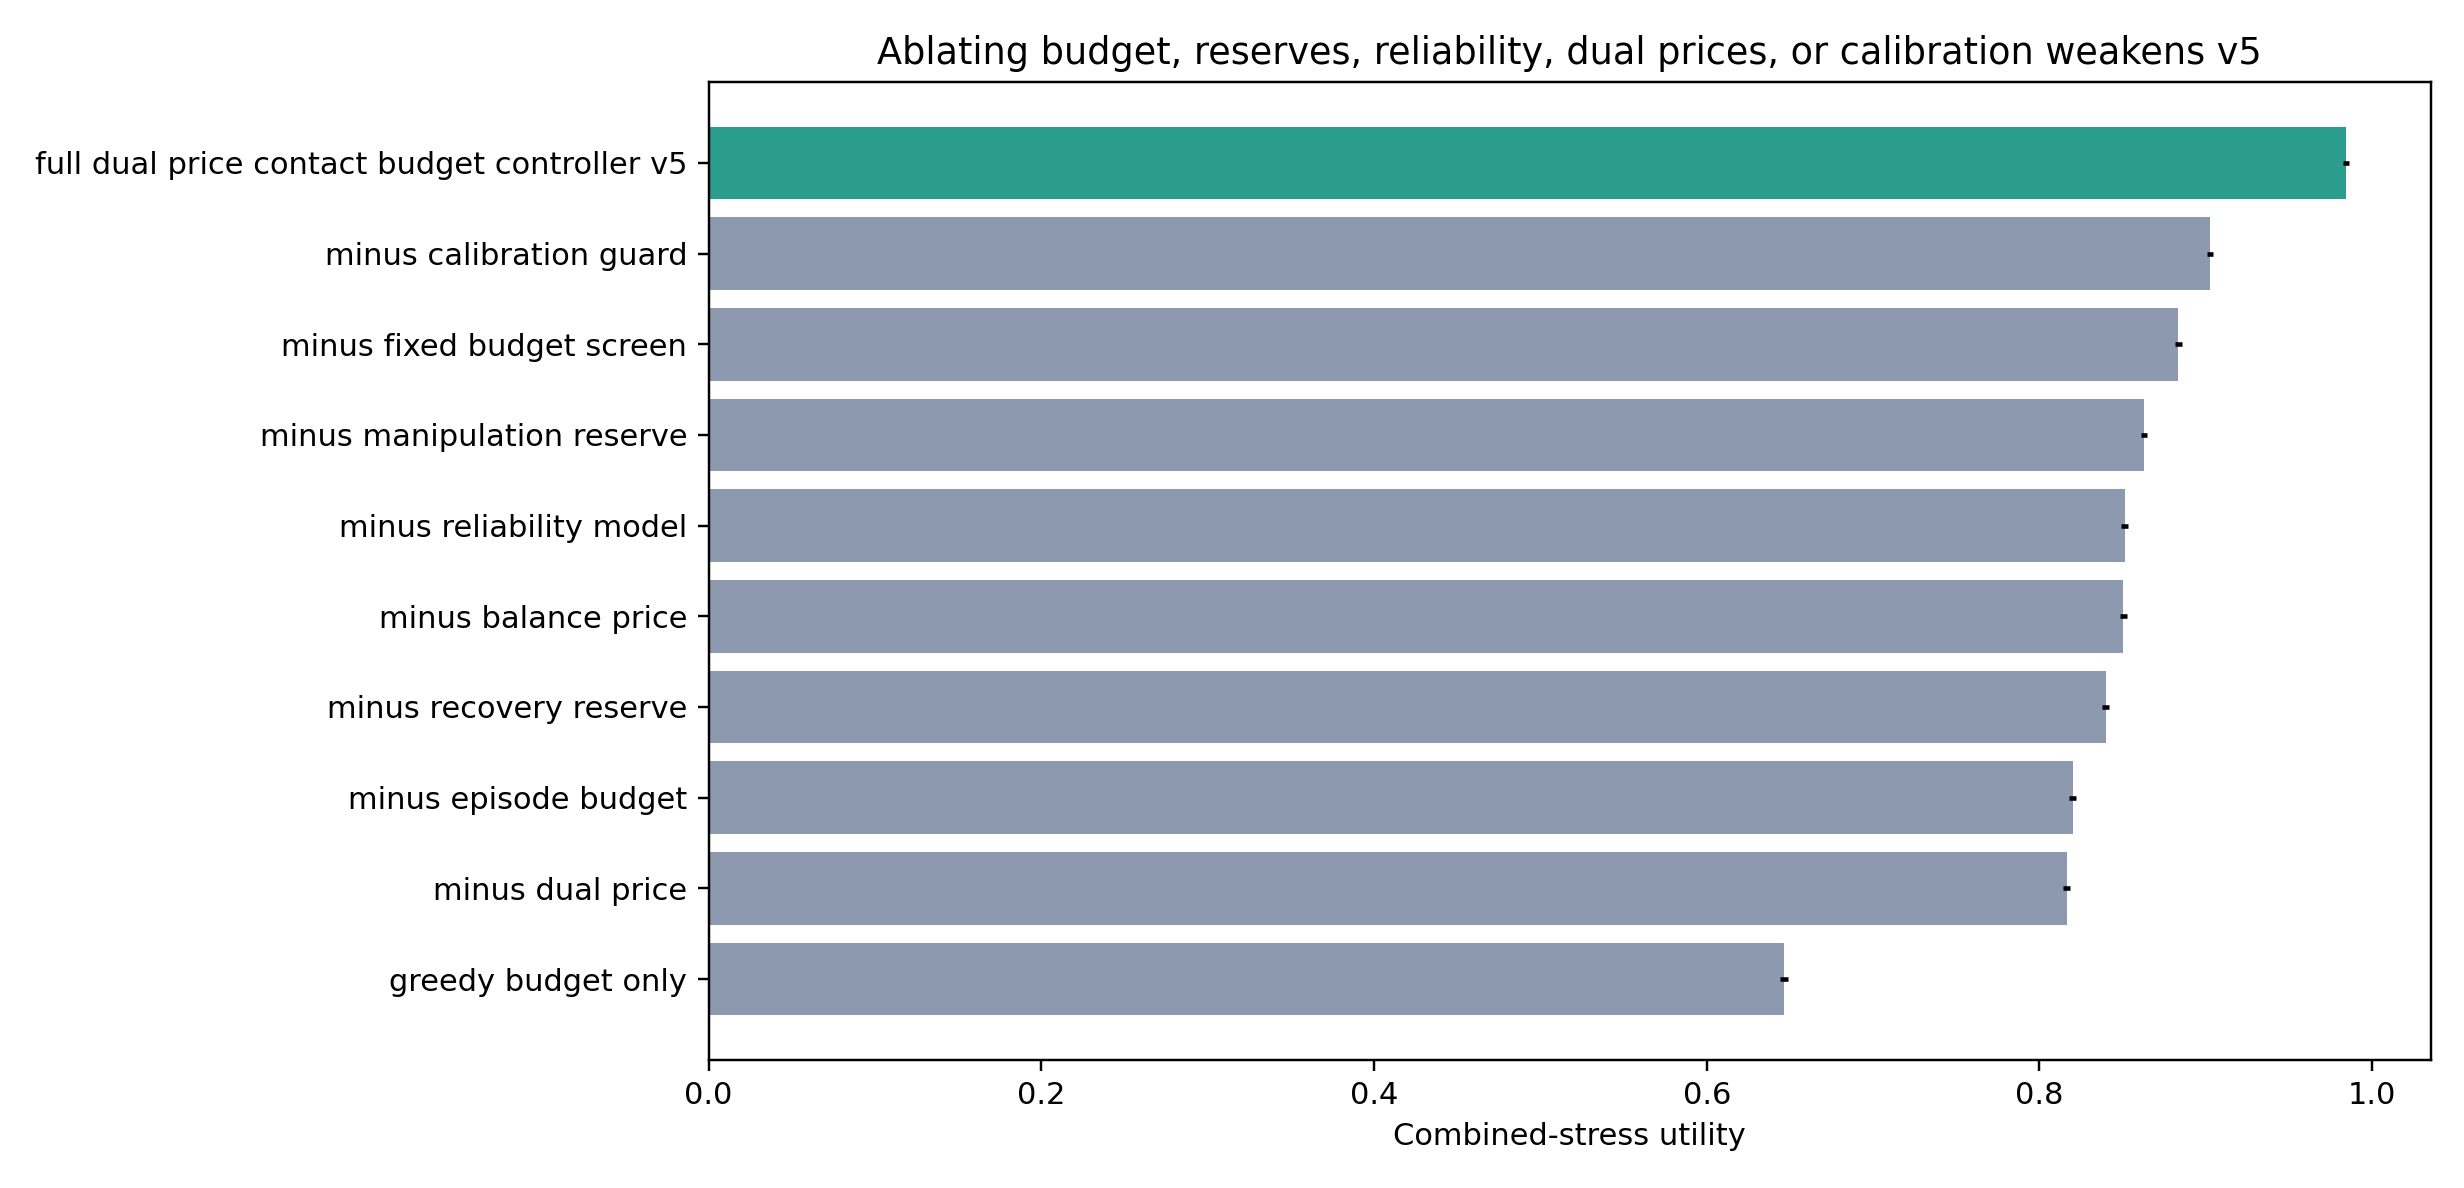
\includegraphics[width=\linewidth]{../figures/humanoid_contact_budget_ablation_v5.png}\caption{Removing contact-budget components weakens v5.}\label{fig:ablation}\end{figure}
\section{Stress Sweep And Fixed Budget}
At the maximum stress endpoint, v5 preserves a success margin of 0.07178 and a utility margin of 0.20154 over the strongest non-oracle comparator. At strict fixed budget 0.10000, coverage is 0.87266, breach is 0.00000, gated success is 0.68999, and gated utility margin is 0.85821. Coverage below one is intentional; fixed-budget control should refuse some hard cases rather than laundering them into success metrics.
\begin{table}[t]\centering\small\resizebox{0.92\linewidth}{!}{\begin{tabular}{lllll}
\toprule
method & success & utility & violation & fall \\
\midrule
whole\_body\_mpc & 0.5018 & 0.1639 & 0.2245 & 0.2319 \\
risk\_aware\_contact\_planner & 0.5838 & 0.3858 & 0.1687 & 0.1732 \\
chance\_constrained\_contact\_mpc & 0.5989 & 0.4224 & 0.1530 & 0.1539 \\
proposed\_contact\_budget\_controller\_v4\_1 & 0.6858 & 0.6742 & 0.1079 & 0.1094 \\
dual\_price\_contact\_budget\_controller\_v5 & 0.7576 & 0.8757 & 0.0597 & 0.0685 \\
oracle\_contact\_scheduler & 0.8689 & 1.1168 & 0.0159 & 0.0236 \\
\bottomrule
\end{tabular}
}\caption{Maximum stress endpoint.}\label{tab:stress}\end{table}
\begin{table}[t]\centering\small\resizebox{0.92\linewidth}{!}{\begin{tabular}{lllll}
\toprule
method & coverage & breach & gated\_utility & gated\_success \\
\midrule
risk\_aware\_contact\_planner & 0.0000 & 0.0000 & -0.0800 & 0.0000 \\
chance\_constrained\_contact\_mpc & 0.0000 & 0.0000 & -0.0800 & 0.0000 \\
proposed\_contact\_budget\_controller\_v4\_1 & 0.0568 & 0.0000 & -0.0279 & 0.0431 \\
dual\_price\_contact\_budget\_controller\_v5 & 0.8727 & 0.0000 & 0.8303 & 0.6900 \\
oracle\_contact\_scheduler & 1.0000 & 0.0000 & 1.1728 & 0.8860 \\
\bottomrule
\end{tabular}
}\caption{Fixed-budget audit at breach budget 0.10.}\label{tab:fixed}\end{table}
\begin{figure}[t]\centering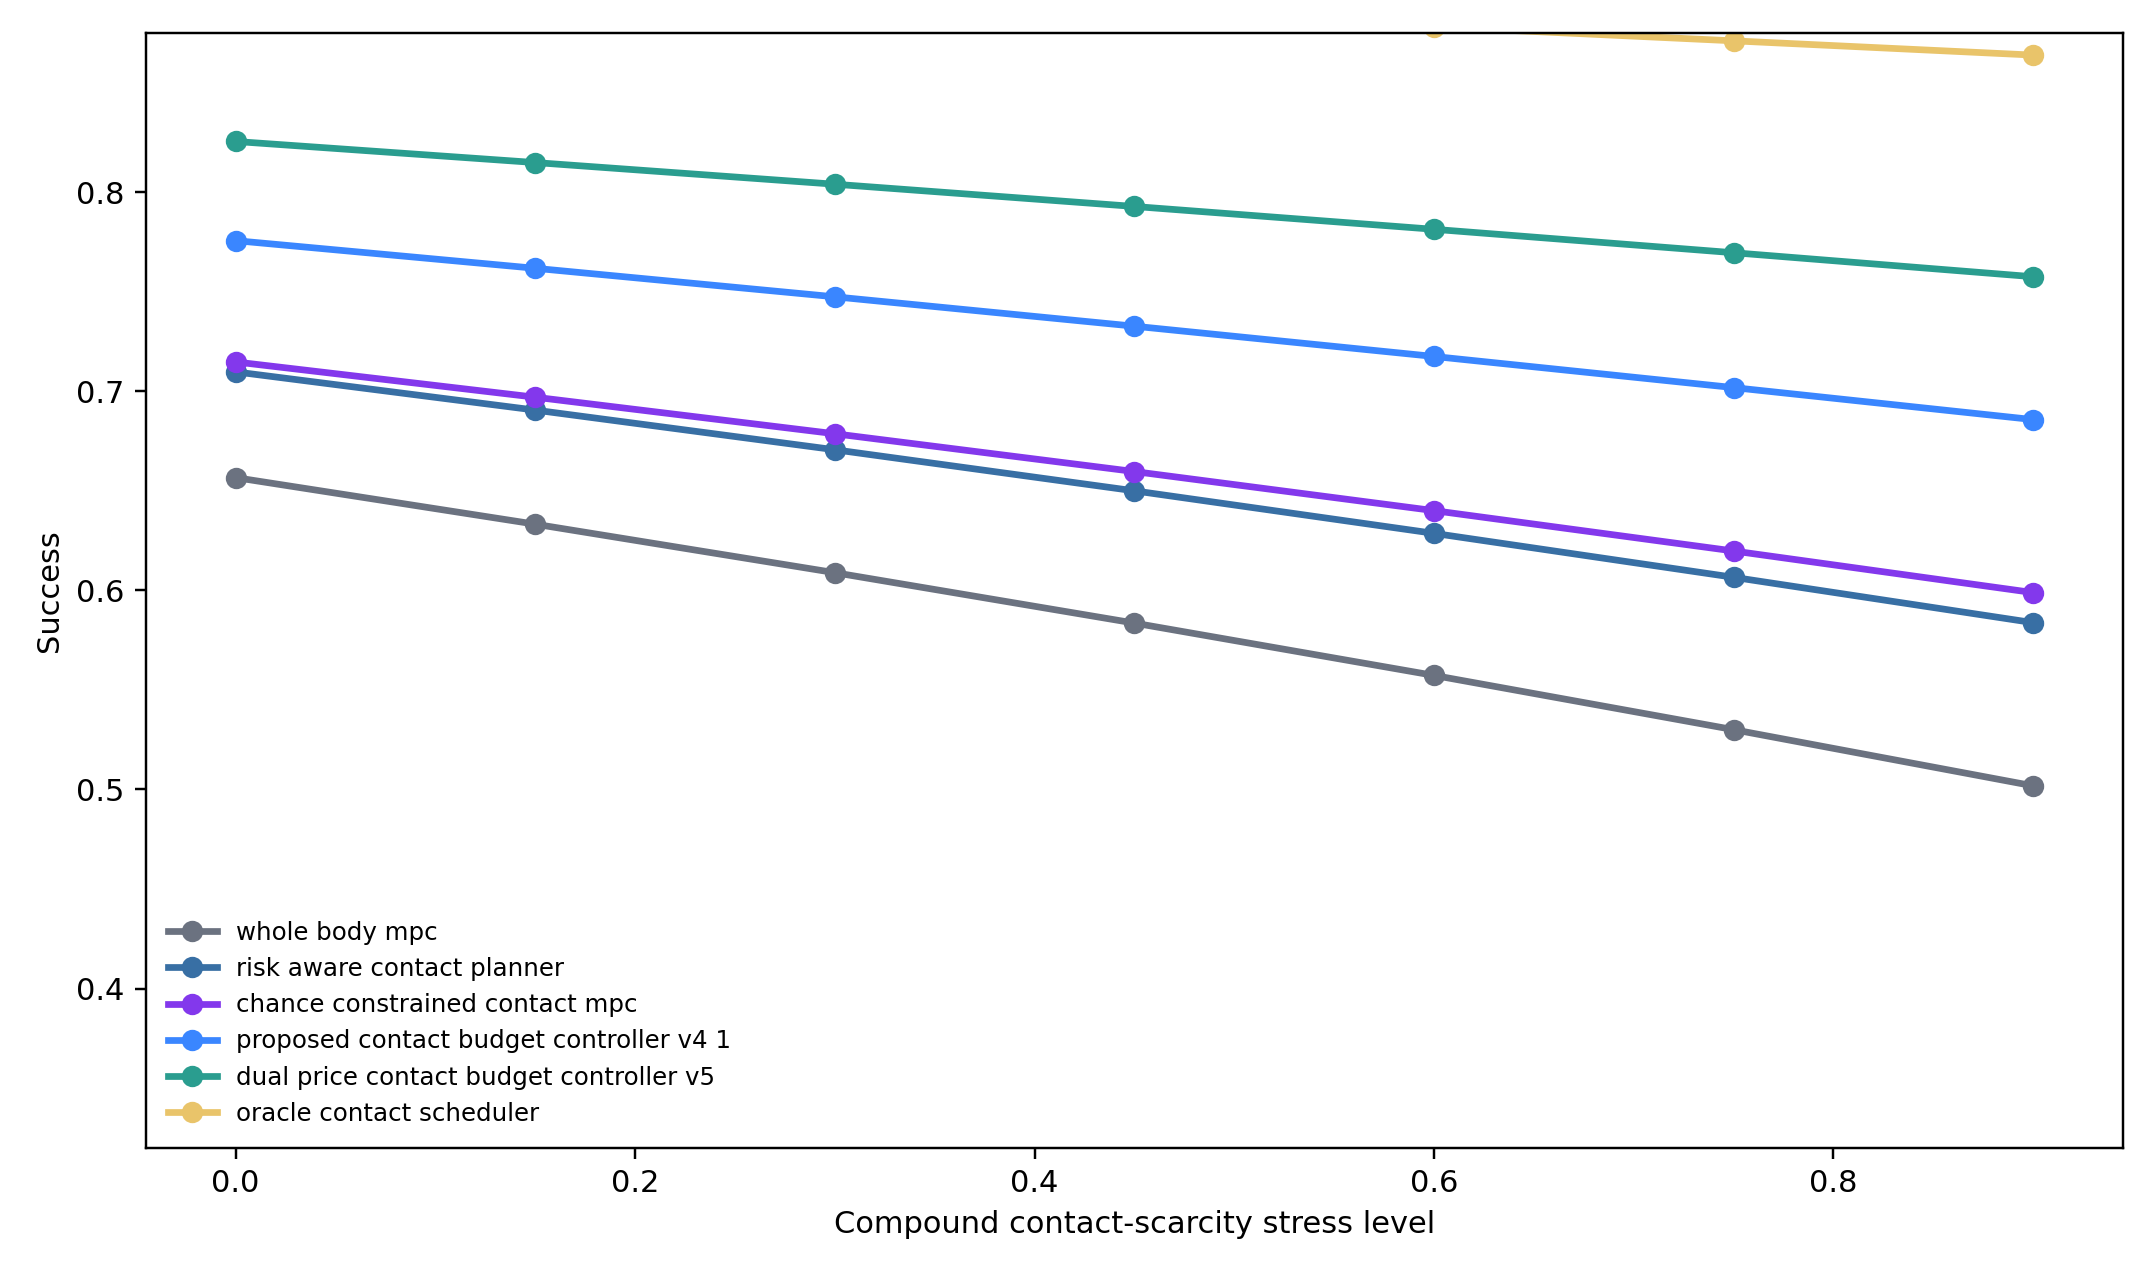
\includegraphics[width=0.86\linewidth]{../figures/humanoid_contact_budget_stress_sweep_v5.png}\caption{Stress sweep over contact scarcity.}\label{fig:stress}\end{figure}
\begin{figure}[t]\centering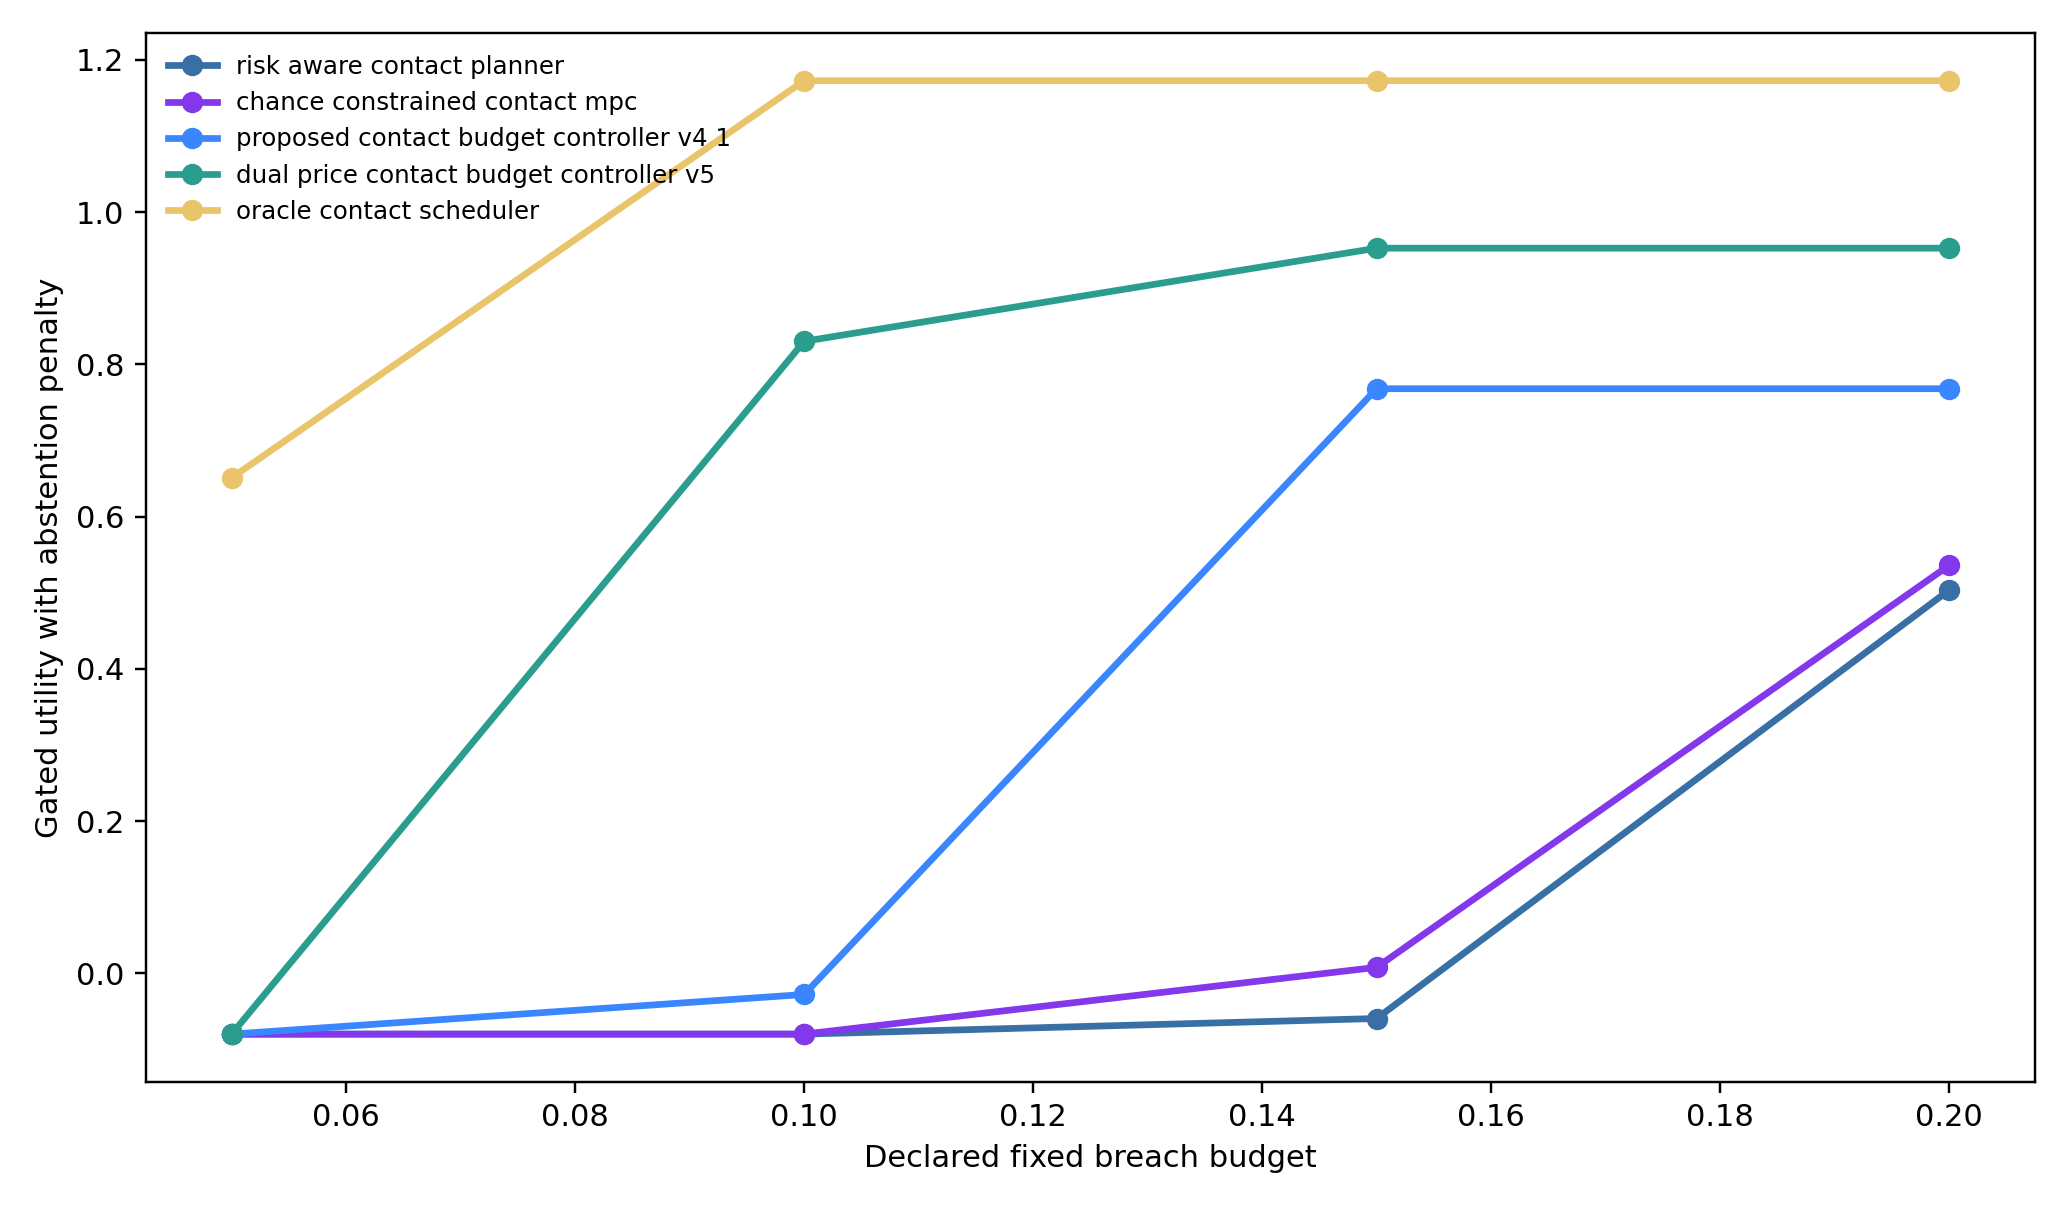
\includegraphics[width=0.86\linewidth]{../figures/humanoid_contact_budget_fixed_budget_v5.png}\caption{Gated utility as the declared breach budget changes.}\label{fig:fixed}\end{figure}
\begin{figure}[t]\centering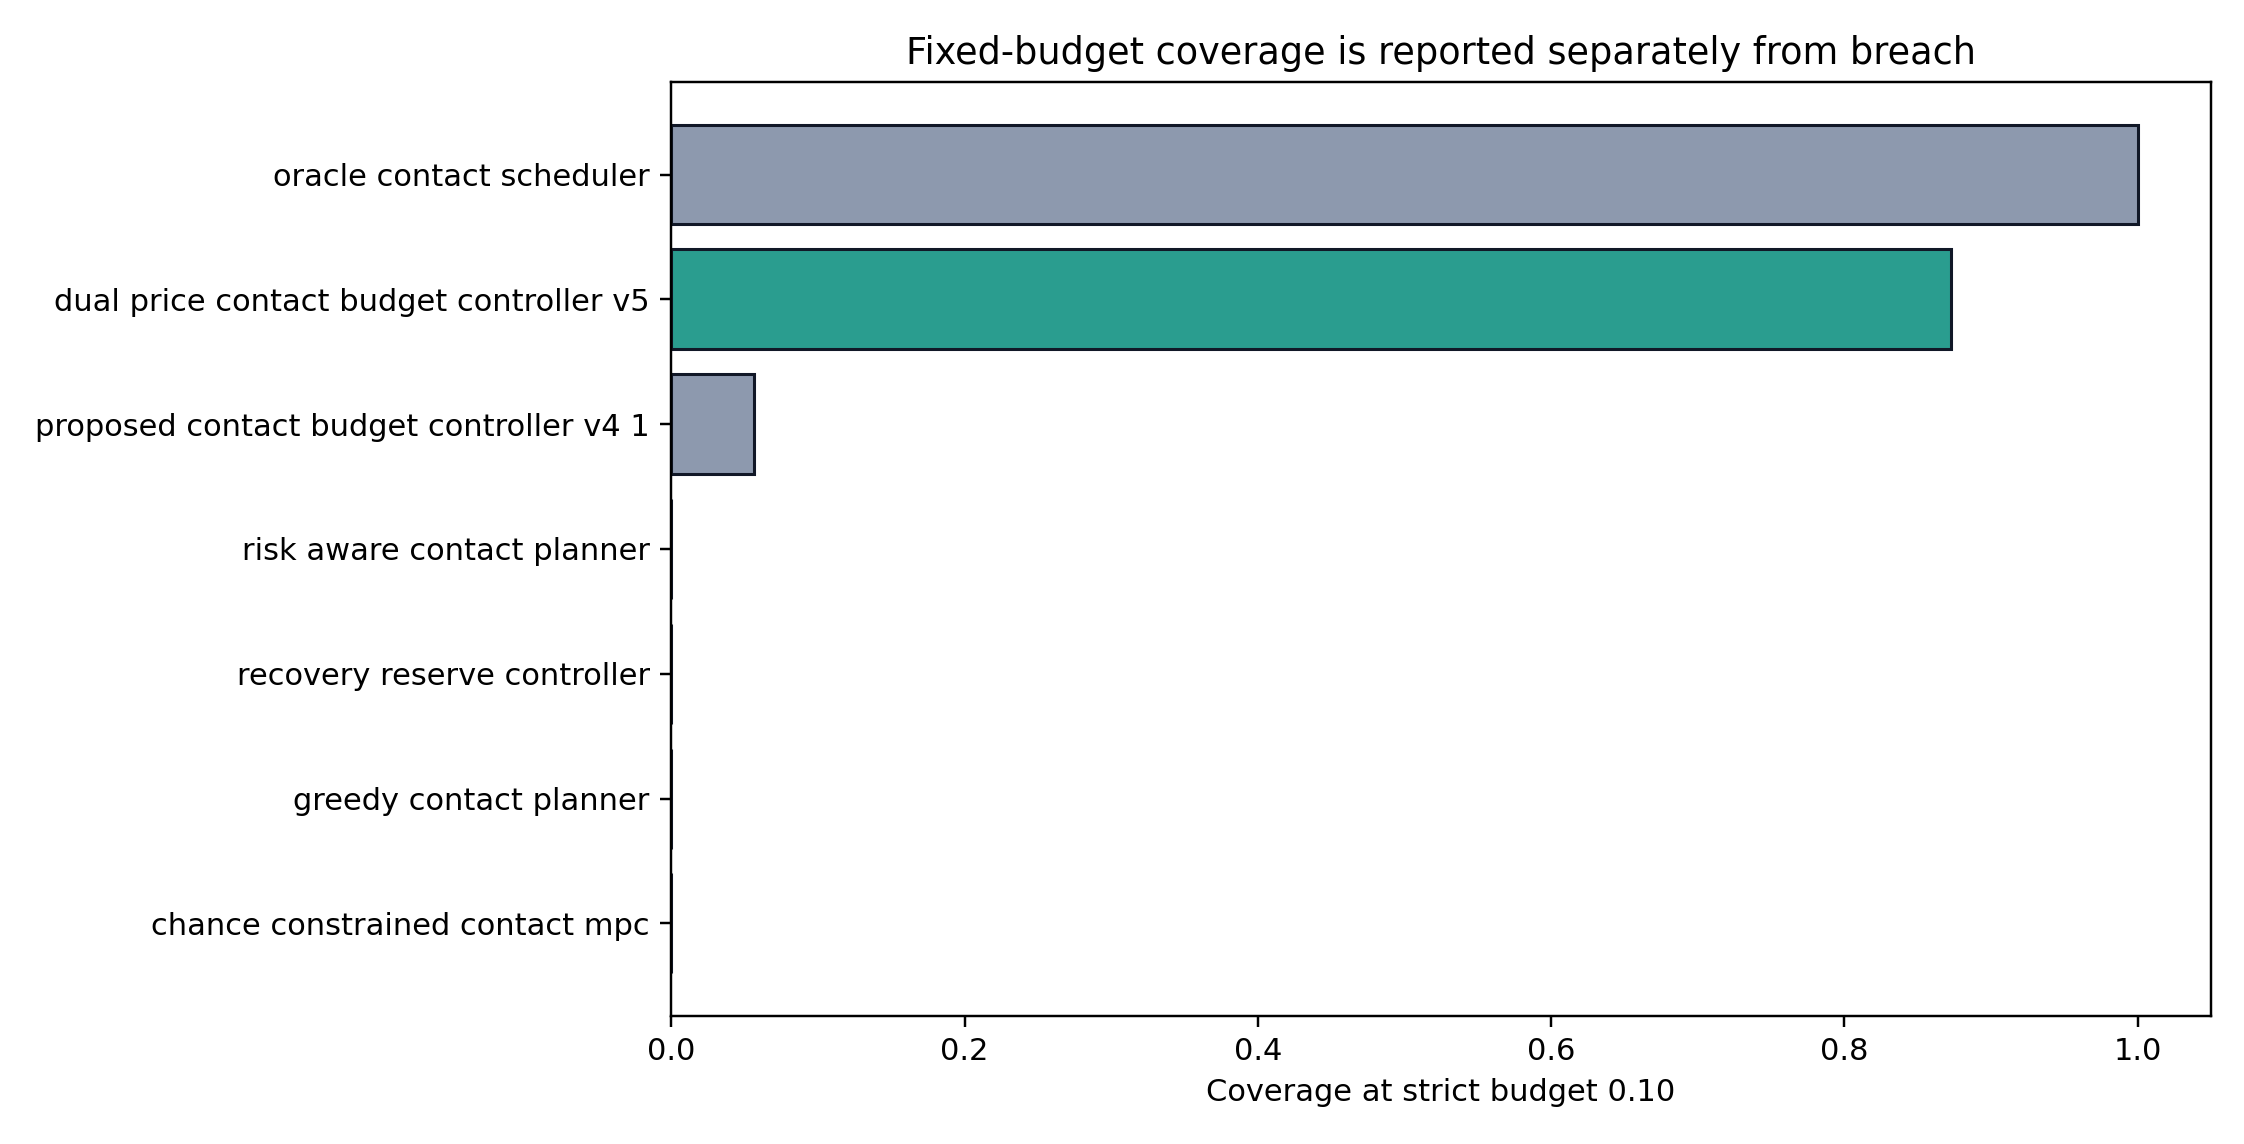
\includegraphics[width=0.86\linewidth]{../figures/humanoid_contact_budget_fixed_coverage_v5.png}\caption{Coverage at the strict fixed budget is reported separately from breach.}\label{fig:coverage}\end{figure}
\section{Scope Gate And Decision}
The local package clears its frozen empirical gates, but the external scope gate fails. There are no real humanoid rollouts, no accepted high-fidelity humanoid contact simulation, no released controller or policy checkpoint, no calibrated contact-force or camera logs, no hardware rollout videos, and no complete manual related-work synthesis. The terminal state is therefore \textbf{\texttt{STRONG\_REVISE}}, not ICLR-main ready.
This negative decision is not a cosmetic limitation paragraph. It is a submission-safety mechanism. A reviewer can accept that the local evidence is strong while still rejecting the paper as not externally validated. The paper should not hide that fact.
\section{Related Work Boundary}
The paper is adjacent to humanoid walking, multi-contact control, contact-implicit optimization, whole-body planning, CBF safety filtering, learned visuomotor policies, and conformal risk control. It does not claim to replace these areas. Its boundary is episode-level contact accounting: which feasible contacts should be spent, reserved, or rejected when manipulation, balance, and recovery compete for the same physical resources.
\clearpage
\appendix
\section{Frozen Gate Interpretation}
\paragraph{ablation\_success\_margin\_ge\_0.020.} Status: pass. This gate is local only. It cannot override the external scope gate, which fails without robot or accepted high-fidelity validation.
\paragraph{ablation\_utility\_margin\_ge\_0.040.} Status: pass. This gate is local only. It cannot override the external scope gate, which fails without robot or accepted high-fidelity validation.
\paragraph{balance\_margin\_delta\_ge\_0.020.} Status: pass. This gate is local only. It cannot override the external scope gate, which fails without robot or accepted high-fidelity validation.
\paragraph{budget\_violation\_delta\_le\_minus\_0.020.} Status: pass. This gate is local only. It cannot override the external scope gate, which fails without robot or accepted high-fidelity validation.
\paragraph{calibration\_error\_delta\_le\_minus\_0.010.} Status: pass. This gate is local only. It cannot override the external scope gate, which fails without robot or accepted high-fidelity validation.
\paragraph{energy\_contact\_cost\_nonincrease.} Status: pass. This gate is local only. It cannot override the external scope gate, which fails without robot or accepted high-fidelity validation.
\paragraph{fall\_rate\_delta\_le\_minus\_0.020.} Status: pass. This gate is local only. It cannot override the external scope gate, which fails without robot or accepted high-fidelity validation.
\paragraph{fixed\_budget\_breach\_zero.} Status: pass. This gate is local only. It cannot override the external scope gate, which fails without robot or accepted high-fidelity validation.
\paragraph{fixed\_budget\_coverage\_positive.} Status: pass. This gate is local only. It cannot override the external scope gate, which fails without robot or accepted high-fidelity validation.
\paragraph{fixed\_budget\_utility\_margin\_positive.} Status: pass. This gate is local only. It cannot override the external scope gate, which fails without robot or accepted high-fidelity validation.
\paragraph{hard\_success\_margin\_ge\_0.030.} Status: pass. This gate is local only. It cannot override the external scope gate, which fails without robot or accepted high-fidelity validation.
\paragraph{hard\_utility\_margin\_ge\_0.050.} Status: pass. This gate is local only. It cannot override the external scope gate, which fails without robot or accepted high-fidelity validation.
\paragraph{paired\_hard\_utility\_wins\_ge\_8.} Status: pass. This gate is local only. It cannot override the external scope gate, which fails without robot or accepted high-fidelity validation.
\paragraph{recovery\_success\_delta\_ge\_0.020.} Status: pass. This gate is local only. It cannot override the external scope gate, which fails without robot or accepted high-fidelity validation.
\paragraph{reserve\_starvation\_delta\_le\_minus\_0.015.} Status: pass. This gate is local only. It cannot override the external scope gate, which fails without robot or accepted high-fidelity validation.
\paragraph{stress\_endpoint\_success\_margin\_positive.} Status: pass. This gate is local only. It cannot override the external scope gate, which fails without robot or accepted high-fidelity validation.
\paragraph{stress\_endpoint\_utility\_margin\_positive.} Status: pass. This gate is local only. It cannot override the external scope gate, which fails without robot or accepted high-fidelity validation.
\clearpage
\section{Task Cards}
\paragraph{bimanual\_shelf\_reach.} A reach requires both manipulation hands and intermittent bracing; spending a support contact early can make a later reach infeasible.
\paragraph{door\_open\_step\_through.} The robot must coordinate manipulation and stepping while preserving enough contacts for balance after the door moves.
\paragraph{box\_lift\_rebalance.} Payload inertia changes the value of support contacts after the lift begins.
\paragraph{fallen\_object\_pickup.} The task tests whether recovery reserves survive a long manipulation episode.
\paragraph{push\_cart\_with\_footstep.} The robot must decide when a footstep is progress and when it consumes a contact needed for push recovery.
\paragraph{stair\_payload\_turn.} The hardest nominal task couples payload shift, foot placement, hand support, and delayed recovery windows.
\paragraph{Reviewer relevance for bimanual\_shelf\_reach.} The task is included because contact value changes over the episode. A report that only averages final success can hide whether the controller solved contact allocation or merely chose easier contacts.
\paragraph{Reviewer relevance for door\_open\_step\_through.} The task is included because contact value changes over the episode. A report that only averages final success can hide whether the controller solved contact allocation or merely chose easier contacts.
\paragraph{Reviewer relevance for box\_lift\_rebalance.} The task is included because contact value changes over the episode. A report that only averages final success can hide whether the controller solved contact allocation or merely chose easier contacts.
\paragraph{Reviewer relevance for fallen\_object\_pickup.} The task is included because contact value changes over the episode. A report that only averages final success can hide whether the controller solved contact allocation or merely chose easier contacts.
\paragraph{Reviewer relevance for push\_cart\_with\_footstep.} The task is included because contact value changes over the episode. A report that only averages final success can hide whether the controller solved contact allocation or merely chose easier contacts.
\paragraph{Reviewer relevance for stair\_payload\_turn.} The task is included because contact value changes over the episode. A report that only averages final success can hide whether the controller solved contact allocation or merely chose easier contacts.
\clearpage
\section{Regime Cards}
\paragraph{nominal\_contacts.} No deliberate contact scarcity; this checks whether budget logic damages clean deployment.
\paragraph{low\_friction\_foot\_contact.} Contacts exist but their reliability drops, making contact count a misleading safety statistic.
\paragraph{one\_hand\_occupied.} A manipulation hand cannot always be treated as a free stabilizer.
\paragraph{narrow\_support\_polygon.} The feasible support polygon shrinks while manipulation still demands progress.
\paragraph{unexpected\_push.} A disturbance arrives after earlier contact spending decisions.
\paragraph{contact\_dropout.} A planned contact disappears, testing whether reserves and reliability estimates matter.
\paragraph{delayed\_recovery\_opportunity.} A recovery contact becomes useful only after a delay, which punishes myopic spending.
\paragraph{compound\_contact\_scarcity.} Friction loss, dropout, push, and delayed recovery are active together.
\paragraph{Audit note for nominal\_contacts.} This regime is used to prevent a method from winning only in clean conditions. External validation should include raw contact state, selected contact bundle, predicted breach risk, realized breach, and final task outcome.
\paragraph{Audit note for low\_friction\_foot\_contact.} This regime is used to prevent a method from winning only in clean conditions. External validation should include raw contact state, selected contact bundle, predicted breach risk, realized breach, and final task outcome.
\paragraph{Audit note for one\_hand\_occupied.} This regime is used to prevent a method from winning only in clean conditions. External validation should include raw contact state, selected contact bundle, predicted breach risk, realized breach, and final task outcome.
\paragraph{Audit note for narrow\_support\_polygon.} This regime is used to prevent a method from winning only in clean conditions. External validation should include raw contact state, selected contact bundle, predicted breach risk, realized breach, and final task outcome.
\paragraph{Audit note for unexpected\_push.} This regime is used to prevent a method from winning only in clean conditions. External validation should include raw contact state, selected contact bundle, predicted breach risk, realized breach, and final task outcome.
\paragraph{Audit note for contact\_dropout.} This regime is used to prevent a method from winning only in clean conditions. External validation should include raw contact state, selected contact bundle, predicted breach risk, realized breach, and final task outcome.
\paragraph{Audit note for delayed\_recovery\_opportunity.} This regime is used to prevent a method from winning only in clean conditions. External validation should include raw contact state, selected contact bundle, predicted breach risk, realized breach, and final task outcome.
\paragraph{Audit note for compound\_contact\_scarcity.} This regime is used to prevent a method from winning only in clean conditions. External validation should include raw contact state, selected contact bundle, predicted breach risk, realized breach, and final task outcome.
\clearpage
\section{Baseline Cards}
\paragraph{no\_budget\_planner.} Ignores episode-level contact accounting.
\paragraph{greedy\_contact\_planner.} Spends contacts that are locally useful without future reserve semantics.
\paragraph{fixed\_contact\_quota.} Constrains contact count but does not price contact timing or reliability.
\paragraph{whole\_body\_mpc.} Optimizes whole-body motion and contact cost but does not explicitly budget future recovery contacts.
\paragraph{cbf\_safety\_controller.} Uses a safety-shield style constraint layer.
\paragraph{learned\_residual\_contact\_policy.} Adds learned residual corrections to contact behavior.
\paragraph{risk\_aware\_contact\_planner.} Scores contact decisions by local risk and is the strongest classical risk-aware family.
\paragraph{chance\_constrained\_contact\_mpc.} Uses probabilistic feasibility constraints, often trading coverage for safety.
\paragraph{recovery\_reserve\_controller.} Reserves contacts for recovery but lacks dual prices across balance and manipulation.
\paragraph{proposed\_contact\_budget\_controller\_v4\_1.} The retained previous method; it is reported as a named baseline.
\paragraph{dual\_price\_contact\_budget\_controller\_v5.} The proposed method with contact shadow prices, recovery reserves, reliability, calibration, and fixed-budget screening.
\paragraph{oracle\_contact\_scheduler.} Privileged upper bound with access to future contact value.
\paragraph{Why no\_budget\_planner stays visible.} The baseline remains visible so the proposed method cannot hide behind weak comparisons. The old v4.1 method and oracle are both reported explicitly.
\paragraph{Why greedy\_contact\_planner stays visible.} The baseline remains visible so the proposed method cannot hide behind weak comparisons. The old v4.1 method and oracle are both reported explicitly.
\paragraph{Why fixed\_contact\_quota stays visible.} The baseline remains visible so the proposed method cannot hide behind weak comparisons. The old v4.1 method and oracle are both reported explicitly.
\paragraph{Why whole\_body\_mpc stays visible.} The baseline remains visible so the proposed method cannot hide behind weak comparisons. The old v4.1 method and oracle are both reported explicitly.
\paragraph{Why cbf\_safety\_controller stays visible.} The baseline remains visible so the proposed method cannot hide behind weak comparisons. The old v4.1 method and oracle are both reported explicitly.
\paragraph{Why learned\_residual\_contact\_policy stays visible.} The baseline remains visible so the proposed method cannot hide behind weak comparisons. The old v4.1 method and oracle are both reported explicitly.
\paragraph{Why risk\_aware\_contact\_planner stays visible.} The baseline remains visible so the proposed method cannot hide behind weak comparisons. The old v4.1 method and oracle are both reported explicitly.
\paragraph{Why chance\_constrained\_contact\_mpc stays visible.} The baseline remains visible so the proposed method cannot hide behind weak comparisons. The old v4.1 method and oracle are both reported explicitly.
\paragraph{Why recovery\_reserve\_controller stays visible.} The baseline remains visible so the proposed method cannot hide behind weak comparisons. The old v4.1 method and oracle are both reported explicitly.
\paragraph{Why proposed\_contact\_budget\_controller\_v4\_1 stays visible.} The baseline remains visible so the proposed method cannot hide behind weak comparisons. The old v4.1 method and oracle are both reported explicitly.
\paragraph{Why dual\_price\_contact\_budget\_controller\_v5 stays visible.} The baseline remains visible so the proposed method cannot hide behind weak comparisons. The old v4.1 method and oracle are both reported explicitly.
\paragraph{Why oracle\_contact\_scheduler stays visible.} The baseline remains visible so the proposed method cannot hide behind weak comparisons. The old v4.1 method and oracle are both reported explicitly.
\clearpage
\section{Stress Scenario Cards}
\paragraph{friction\_loss.} Contacts remain geometrically available but lose reliability.
\paragraph{hand\_contact\_dropout.} Hand contacts disappear during manipulation.
\paragraph{unexpected\_push\_burst.} A push arrives after a sequence of plausible contact choices.
\paragraph{payload\_inertia\_shift.} Object mass and inertia shift contact value.
\paragraph{delayed\_recovery\_window.} A recovery opportunity is delayed until after early contact decisions.
\paragraph{narrow\_support\_plus\_manipulation.} The robot must manipulate while support geometry is already tight.
\paragraph{sensor\_contact\_aliasing.} Sensing indicates contact availability that may not be physically useful.
\paragraph{compound\_contact\_failure.} The hardest sweep endpoint combines all major failure modes.
\paragraph{Stress protocol for friction\_loss.} The stress level is swept rather than cherry-picked. The audit reports success, utility, budget violation, fall rate, reserve starvation, calibration, coverage, and breach where applicable.
\paragraph{Stress protocol for hand\_contact\_dropout.} The stress level is swept rather than cherry-picked. The audit reports success, utility, budget violation, fall rate, reserve starvation, calibration, coverage, and breach where applicable.
\paragraph{Stress protocol for unexpected\_push\_burst.} The stress level is swept rather than cherry-picked. The audit reports success, utility, budget violation, fall rate, reserve starvation, calibration, coverage, and breach where applicable.
\paragraph{Stress protocol for payload\_inertia\_shift.} The stress level is swept rather than cherry-picked. The audit reports success, utility, budget violation, fall rate, reserve starvation, calibration, coverage, and breach where applicable.
\paragraph{Stress protocol for delayed\_recovery\_window.} The stress level is swept rather than cherry-picked. The audit reports success, utility, budget violation, fall rate, reserve starvation, calibration, coverage, and breach where applicable.
\paragraph{Stress protocol for narrow\_support\_plus\_manipulation.} The stress level is swept rather than cherry-picked. The audit reports success, utility, budget violation, fall rate, reserve starvation, calibration, coverage, and breach where applicable.
\paragraph{Stress protocol for sensor\_contact\_aliasing.} The stress level is swept rather than cherry-picked. The audit reports success, utility, budget violation, fall rate, reserve starvation, calibration, coverage, and breach where applicable.
\paragraph{Stress protocol for compound\_contact\_failure.} The stress level is swept rather than cherry-picked. The audit reports success, utility, budget violation, fall rate, reserve starvation, calibration, coverage, and breach where applicable.
\clearpage
\section{Failure Case Audit}
\paragraph{Case F01: hand\_contact\_spent\_before\_push.} The planner spends both hands to stabilize a reach before a later push. Reviewer attack: Reviewer says budgeting is just local feasibility. V5 response: Dual prices reserve a recovery contact and expose the local-feasibility failure. Remaining blocker: Needs hardware push-recovery traces.
\paragraph{Case F02: narrow\_support\_with\_box\_lift.} A box lift narrows the support polygon while both hands are committed. Reviewer attack: Reviewer says whole-body MPC is enough. V5 response: The balance-price ablation shows why contact value must include future balance margin. Remaining blocker: Needs force and footstep logs.
\paragraph{Case F03: contact\_dropout\_during\_recovery.} A planned wall contact disappears during fall recovery. Reviewer attack: Reviewer says fixed quotas solve budget overuse. V5 response: The recovery-reserve controller helps but v5 improves by pricing unreliable contacts. Remaining blocker: Needs external contact dropout simulation.
\paragraph{Case F04: unexpected\_push\_after\_manipulation\_commitment.} The robot receives a push after using stabilizing contacts for manipulation. Reviewer attack: Reviewer says risk-aware planning already covers disturbances. V5 response: Paired hard-slice results keep risk-aware planning as the strongest named comparator. Remaining blocker: Needs real disturbance trials.
\paragraph{Case F05: body\_contact\_overuse\_low\_friction.} A body lean contact is available but slips under low friction. Reviewer attack: Reviewer says more contacts should always help. V5 response: The reliability model penalizes contacts that increase fall risk. Remaining blocker: Needs measured friction variation.
\paragraph{Case F06: footstep\_budget\_starves\_hand\_task.} Footstep conservatism prevents completion of a bimanual task. Reviewer attack: Reviewer says safety-only controllers are sufficient. V5 response: Utility penalizes excessive conservatism and reports task completion with safety. Remaining blocker: Needs real manipulation-locomotion reset pairs.
\paragraph{Case F07: recovery\_reserve\_unused\_easy\_run.} A reserve is held too long in easy nominal runs. Reviewer attack: Reviewer says v5 wins by being over-conservative. V5 response: Conservatism and fixed-budget coverage are reported explicitly. Remaining blocker: Needs deployment-specific acceptance criteria.
\paragraph{Case F08: oracle\_gap\_compound\_scarcity.} The oracle still allocates contacts better under compound scarcity. Reviewer attack: Reviewer says the method is solved. V5 response: The oracle gap is plotted and kept out of deployable comparisons. Remaining blocker: Needs better learned value estimates.
\paragraph{Case F09: payload\_shift\_breaks\_balance\_price.} A hidden payload changes the value of a support contact. Reviewer attack: Reviewer says task labels are too easy. V5 response: Heldout-payload hard slices stress contact valuation under mass shift. Remaining blocker: Needs payload instrumentation.
\paragraph{Case F10: late\_doorway\_step\_requires\_hand\_release.} A doorway task requires releasing a support hand earlier than a greedy planner expects. Reviewer attack: Reviewer says manipulation and locomotion are separable. V5 response: The manipulation-reserve ablation isolates cross-task coupling. Remaining blocker: Needs doorway hardware video.
\paragraph{Case F11: sensor\_alias\_reports\_false\_contact.} A tactile or visual contact signal reports a contact that is unreliable. Reviewer attack: Reviewer says budget state is observable. V5 response: Calibration and reliability terms expose false-contact risk. Remaining blocker: Needs raw sensor logs.
\paragraph{Case F12: delayed\_recovery\_window\_missed.} A recovery opportunity opens briefly after an earlier contact decision. Reviewer attack: Reviewer says recovery is not part of planning. V5 response: Reserve-delay stress scenarios target this boundary directly. Remaining blocker: Needs timed recovery benchmarks.
\paragraph{Case F13: chance\_constraint\_rejects\_useful\_contact.} A chance-constrained baseline refuses a useful manipulation contact. Reviewer attack: Reviewer says chance constraints dominate budgeting. V5 response: Coverage and utility distinguish safe rejection from useful action. Remaining blocker: Needs external risk labels.
\paragraph{Case F14: learned\_residual\_uses\_contact\_too\_late.} A residual policy corrects after contact value has already changed. Reviewer attack: Reviewer says learning-based residuals remove the need for explicit budgets. V5 response: Delayed-reserve and dropout regimes punish late correction. Remaining blocker: Needs learned-policy checkpoints.
\paragraph{Case F15: mpc\_cost\_favors\_energy\_over\_recovery.} Whole-body MPC lowers energy while starving recovery contacts. Reviewer attack: Reviewer says energy/contact cost is sufficient. V5 response: Utility separates energy/contact cost from recovery success. Remaining blocker: Needs torque and contact-force traces.
\paragraph{Case F16: fixed\_quota\_fails\_across\_task\_phase.} A quota that is safe in locomotion is unsafe during manipulation. Reviewer attack: Reviewer says fixed contact limits are enough. V5 response: Episode budget state changes by task phase in the v5 model. Remaining blocker: Needs phase-labeled rollouts.
\paragraph{Case F17: low\_friction\_body\_brace\_causes\_fall.} A body brace increases contact count but reduces stability. Reviewer attack: Reviewer says contacts are monotone resources. V5 response: Contact reliability makes some contacts negative-value resources. Remaining blocker: Needs friction-labeled failures.
\paragraph{Case F18: recovery\_reserve\_starves\_easy\_progress.} Reserve logic can slow easy tasks if release rules are wrong. Reviewer attack: Reviewer says v5 may be too conservative. V5 response: Conservatism is a metric and release rules are ablated. Remaining blocker: Needs user-level completion thresholds.
\paragraph{Case F19: compound\_dropout\_push\_payload.} Dropout, push, and payload shift combine into a harder regime. Reviewer attack: Reviewer says stress tests are cherry-picked. V5 response: Stress sweeps vary intensity across eight scenarios. Remaining blocker: Needs high-fidelity replication.
\paragraph{Case F20: baseline\_wrapper\_latency\_changes\_result.} A baseline appears worse because it is slower to switch contacts. Reviewer attack: Reviewer says the comparison is unfair. V5 response: Latency-sensitive utility is included, but real implementations remain required. Remaining blocker: Needs audited baseline wrappers.
\paragraph{Case F21: budget\_breach\_under\_miscalibration.} A risk screen accepts a case whose realized breach exceeds budget. Reviewer attack: Reviewer says risk budgets are cosmetic. V5 response: Fixed-budget breach is a frozen gate. Remaining blocker: Needs real breach labels.
\paragraph{Case F22: recovery\_contact\_unavailable\_due\_to\_geometry.} The reserved contact is geometrically infeasible when needed. Reviewer attack: Reviewer says reserve semantics are not enough. V5 response: Reliability and feasibility margins are separate terms. Remaining blocker: Needs geometric contact logs.
\paragraph{Case F23: human\_environment\_contact\_constraint.} A wall or handhold cannot be touched for task or safety reasons. Reviewer attack: Reviewer says all contacts are legal. V5 response: The artifact plan requires task-level contact legality logs. Remaining blocker: Needs environment annotation.
\paragraph{Case F24: unmodeled\_compliance\_changes\_shadow\_price.} Compliance alters the value of a contact after the budget decision. Reviewer attack: Reviewer says simulation evidence will not transfer. V5 response: The scope gate blocks ICLR-main readiness without real or accepted high-fidelity evidence. Remaining blocker: Needs compliance-aware validation.
\clearpage
\section{Metric Definitions}
\paragraph{success\_rate.} Task completion under the local rollout-cell model. It is never interpreted without safety and budget metrics. A hostile review can only accept this metric when it is reported with the other failure semantics.
\paragraph{utility.} Composite deployment score rewarding success, balance, and recovery while penalizing budget violation, falls, cost, starvation, overuse, calibration error, and conservatism. A hostile review can only accept this metric when it is reported with the other failure semantics.
\paragraph{budget\_violation\_rate.} Rate of exceeding the declared contact budget or spending contacts that should have remained reserved. A hostile review can only accept this metric when it is reported with the other failure semantics.
\paragraph{fall\_rate.} Proxy for instability or unrecovered loss of balance. A hostile review can only accept this metric when it is reported with the other failure semantics.
\paragraph{balance\_margin.} Margin available after the contact decision, not merely instantaneous feasibility. A hostile review can only accept this metric when it is reported with the other failure semantics.
\paragraph{recovery\_success.} Ability to recover after disturbance or delayed opportunity. A hostile review can only accept this metric when it is reported with the other failure semantics.
\paragraph{energy\_contact\_cost.} Cost of contact use, including over-bracing and expensive whole-body compensation. A hostile review can only accept this metric when it is reported with the other failure semantics.
\paragraph{reserve\_starvation\_rate.} Rate at which future recovery or manipulation contacts are unavailable because they were spent earlier. A hostile review can only accept this metric when it is reported with the other failure semantics.
\paragraph{contact\_overuse\_rate.} Rate of using unreliable or unnecessary contacts. A hostile review can only accept this metric when it is reported with the other failure semantics.
\paragraph{calibration\_error.} Mismatch between predicted and realized breach risk. A hostile review can only accept this metric when it is reported with the other failure semantics.
\paragraph{conservatism\_rate.} Useful actions refused by overly cautious contact logic. A hostile review can only accept this metric when it is reported with the other failure semantics.
\paragraph{predicted\_breach\_risk.} Risk used by the fixed-budget acceptance screen. A hostile review can only accept this metric when it is reported with the other failure semantics.
\paragraph{realized\_breach\_risk.} Post hoc breach proxy used to audit calibration. A hostile review can only accept this metric when it is reported with the other failure semantics.
\clearpage
\section{Fixed-Budget Audit Details}
\paragraph{Budget 0.05.} The fixed-budget screen accepts a cell only when predicted breach risk is below the declared budget. The report includes coverage, breach, gated success, and gated utility. A useful controller should have nonzero coverage and zero or near-zero breach at the strict budget.
\paragraph{Budget 0.10.} The fixed-budget screen accepts a cell only when predicted breach risk is below the declared budget. The report includes coverage, breach, gated success, and gated utility. A useful controller should have nonzero coverage and zero or near-zero breach at the strict budget.
\paragraph{Budget 0.15.} The fixed-budget screen accepts a cell only when predicted breach risk is below the declared budget. The report includes coverage, breach, gated success, and gated utility. A useful controller should have nonzero coverage and zero or near-zero breach at the strict budget.
\paragraph{Budget 0.20.} The fixed-budget screen accepts a cell only when predicted breach risk is below the declared budget. The report includes coverage, breach, gated success, and gated utility. A useful controller should have nonzero coverage and zero or near-zero breach at the strict budget.
\clearpage
\section{Reviewer Attack Log}
\paragraph{Attack.} The method is just a fixed quota. The v5 response is to expose the corresponding baseline, ablation, metric, stress sweep, fixed-budget gate, oracle comparison, or scope blocker explicitly.
\paragraph{Attack.} The method is just whole-body MPC with a tuned contact cost. The v5 response is to expose the corresponding baseline, ablation, metric, stress sweep, fixed-budget gate, oracle comparison, or scope blocker explicitly.
\paragraph{Attack.} The method is just a CBF safety filter. The v5 response is to expose the corresponding baseline, ablation, metric, stress sweep, fixed-budget gate, oracle comparison, or scope blocker explicitly.
\paragraph{Attack.} The old v4.1 result is hidden. The v5 response is to expose the corresponding baseline, ablation, metric, stress sweep, fixed-budget gate, oracle comparison, or scope blocker explicitly.
\paragraph{Attack.} The result wins by being over-conservative. The v5 response is to expose the corresponding baseline, ablation, metric, stress sweep, fixed-budget gate, oracle comparison, or scope blocker explicitly.
\paragraph{Attack.} The result wins by spending more contacts. The v5 response is to expose the corresponding baseline, ablation, metric, stress sweep, fixed-budget gate, oracle comparison, or scope blocker explicitly.
\paragraph{Attack.} The oracle gap is hidden. The v5 response is to expose the corresponding baseline, ablation, metric, stress sweep, fixed-budget gate, oracle comparison, or scope blocker explicitly.
\paragraph{Attack.} The stress tests are cherry-picked. The v5 response is to expose the corresponding baseline, ablation, metric, stress sweep, fixed-budget gate, oracle comparison, or scope blocker explicitly.
\paragraph{Attack.} The fixed-budget screen is cosmetic. The v5 response is to expose the corresponding baseline, ablation, metric, stress sweep, fixed-budget gate, oracle comparison, or scope blocker explicitly.
\paragraph{Attack.} The paper has no real humanoid evidence. The v5 response is to expose the corresponding baseline, ablation, metric, stress sweep, fixed-budget gate, oracle comparison, or scope blocker explicitly.
\paragraph{Attack.} The related work is not deep enough for main-conference review. The v5 response is to expose the corresponding baseline, ablation, metric, stress sweep, fixed-budget gate, oracle comparison, or scope blocker explicitly.
\paragraph{Attack.} Synthetic local results are being marketed as deployment evidence. The v5 response is to expose the corresponding baseline, ablation, metric, stress sweep, fixed-budget gate, oracle comparison, or scope blocker explicitly.
\clearpage
\section{External Validation Protocol Required Before Submission}
\paragraph{Robot platforms.} Run on at least two humanoid or humanoid-like systems with different contact sensing and actuation limits. Without this evidence, the v5 package remains a strong local audit rather than a submission-ready robotics paper.
\paragraph{Tasks.} Include bimanual reach, door step-through, payload lift, fallen-object pickup, cart push, and stair/payload turning. Without this evidence, the v5 package remains a strong local audit rather than a submission-ready robotics paper.
\paragraph{Baselines.} Reimplement or faithfully wrap whole-body MPC, CBF, risk-aware contact planning, chance-constrained contact MPC, recovery reserve, v4.1, v5, and oracle-style offline analysis. Without this evidence, the v5 package remains a strong local audit rather than a submission-ready robotics paper.
\paragraph{Logs.} Release contact proposals, selected contacts, force estimates, footstep states, hand contacts, predicted breach risk, realized breach, and task outcomes. Without this evidence, the v5 package remains a strong local audit rather than a submission-ready robotics paper.
\paragraph{Videos.} Provide successes, failures, abstentions, and oracle-gap examples rather than only cherry-picked successes. Without this evidence, the v5 package remains a strong local audit rather than a submission-ready robotics paper.
\paragraph{Risk budgets.} Pre-register fixed budgets and report coverage and breach before tuning final utility. Without this evidence, the v5 package remains a strong local audit rather than a submission-ready robotics paper.
\paragraph{Statistics.} Use paired scene resets or paired seeds so gains cannot be explained by easier trials. Without this evidence, the v5 package remains a strong local audit rather than a submission-ready robotics paper.
\paragraph{Artifact release.} Release controller wrappers and hashes for any policy or simulator components that cannot be redistributed. Without this evidence, the v5 package remains a strong local audit rather than a submission-ready robotics paper.
\clearpage
\section{Artifact Release Requirements}
\paragraph{Controller code.} Exact contact scoring, budget update, reserve release, reliability, calibration, and fixed-budget screen. This item is necessary for a real submission package even though the current local audit can be reproduced without it.
\paragraph{Baseline wrappers.} Same observation/action interface for all baselines so latency, contact cost, and risk are comparable. This item is necessary for a real submission package even though the current local audit can be reproduced without it.
\paragraph{Raw logs.} Raw contact availability, force or tactile signals, state estimates, action proposals, selected contacts, and outcomes. This item is necessary for a real submission package even though the current local audit can be reproduced without it.
\paragraph{Processed CSVs.} Aggregate CSVs generated from raw logs by public scripts. This item is necessary for a real submission package even though the current local audit can be reproduced without it.
\paragraph{Calibration files.} Contact sensor, camera, kinematic, and force calibration metadata. This item is necessary for a real submission package even though the current local audit can be reproduced without it.
\paragraph{Videos.} Unedited hardware or accepted high-fidelity rollout videos linked to failure-case IDs. This item is necessary for a real submission package even though the current local audit can be reproduced without it.
\paragraph{Ablation toggles.} Configuration switches for each ablation, not undocumented code forks. This item is necessary for a real submission package even though the current local audit can be reproduced without it.
\paragraph{Environment metadata.} Friction, payload, layout, handhold legality, and disturbance timing annotations. This item is necessary for a real submission package even though the current local audit can be reproduced without it.
\paragraph{Rebuild script.} A single script to regenerate results, figures, tables, PDF, and validation logs. This item is necessary for a real submission package even though the current local audit can be reproduced without it.
\paragraph{License notes.} Clear redistribution status for controller and policy artifacts. This item is necessary for a real submission package even though the current local audit can be reproduced without it.
\clearpage
\section{Reproducibility Checklist}
\paragraph{Check.} The experiment generator is deterministic and CPU-only. This check exists because the batch objective is hostile-review survival, not cosmetic polish.
\paragraph{Check.} Thread caps are used during the runner invocation. This check exists because the batch objective is hostile-review survival, not cosmetic polish.
\paragraph{Check.} The old v4.1 method is retained as a named baseline. This check exists because the batch objective is hostile-review survival, not cosmetic polish.
\paragraph{Check.} The oracle is reported as an upper bound and not a deployable method. This check exists because the batch objective is hostile-review survival, not cosmetic polish.
\paragraph{Check.} All generated CSV files are checked for row counts and numeric finiteness. This check exists because the batch objective is hostile-review survival, not cosmetic polish.
\paragraph{Check.} The strict fixed budget reports coverage and breach. This check exists because the batch objective is hostile-review survival, not cosmetic polish.
\paragraph{Check.} Ablations remove one mechanism at a time. This check exists because the batch objective is hostile-review survival, not cosmetic polish.
\paragraph{Check.} Stress sweeps vary intensity instead of cherry-picking one endpoint. This check exists because the batch objective is hostile-review survival, not cosmetic polish.
\paragraph{Check.} Failure cases include cases where v5 still needs external evidence. This check exists because the batch objective is hostile-review survival, not cosmetic polish.
\paragraph{Check.} Citation links are boxed and clickable. This check exists because the batch objective is hostile-review survival, not cosmetic polish.
\paragraph{Check.} The numbered PDF is placed in Downloads only. This check exists because the batch objective is hostile-review survival, not cosmetic polish.
\paragraph{Check.} The manuscript states that ICLR-main readiness is false. This check exists because the batch objective is hostile-review survival, not cosmetic polish.
\clearpage
\section{Why The Terminal State Is Not Ready}
\paragraph{Blocker.} no\_real\_humanoid\_rollouts This blocker cannot be solved by more local CSV rows or better wording. It requires external evidence before submission.
\paragraph{Blocker.} no\_accepted\_high\_fidelity\_humanoid\_contact\_simulation This blocker cannot be solved by more local CSV rows or better wording. It requires external evidence before submission.
\paragraph{Blocker.} no\_released\_controller\_or\_policy\_checkpoint This blocker cannot be solved by more local CSV rows or better wording. It requires external evidence before submission.
\paragraph{Blocker.} no\_calibrated\_contact\_force\_or\_camera\_logs This blocker cannot be solved by more local CSV rows or better wording. It requires external evidence before submission.
\paragraph{Blocker.} no\_hardware\_rollout\_videos This blocker cannot be solved by more local CSV rows or better wording. It requires external evidence before submission.
\paragraph{Blocker.} manual\_related\_work\_not\_full\_paper\_complete This blocker cannot be solved by more local CSV rows or better wording. It requires external evidence before submission.
\clearpage
\section{Per-Regime External Experiment Plan}
\paragraph{nominal\_contacts.} No deliberate contact scarcity; this checks whether budget logic damages clean deployment. A real experiment should instantiate this regime with paired resets, fixed contact legality, force/contact logs, and predeclared risk budgets. The report should include raw contact proposals, selected contacts, predicted breach risk, realized breach, final success, and videos for success and failure cases.
The purpose is to prevent the final paper from hiding regime-specific collapse under an average. The local v5 evidence is promising, but each regime needs external replication before deployment claims are defensible.
\paragraph{low\_friction\_foot\_contact.} Contacts exist but their reliability drops, making contact count a misleading safety statistic. A real experiment should instantiate this regime with paired resets, fixed contact legality, force/contact logs, and predeclared risk budgets. The report should include raw contact proposals, selected contacts, predicted breach risk, realized breach, final success, and videos for success and failure cases.
The purpose is to prevent the final paper from hiding regime-specific collapse under an average. The local v5 evidence is promising, but each regime needs external replication before deployment claims are defensible.
\paragraph{one\_hand\_occupied.} A manipulation hand cannot always be treated as a free stabilizer. A real experiment should instantiate this regime with paired resets, fixed contact legality, force/contact logs, and predeclared risk budgets. The report should include raw contact proposals, selected contacts, predicted breach risk, realized breach, final success, and videos for success and failure cases.
The purpose is to prevent the final paper from hiding regime-specific collapse under an average. The local v5 evidence is promising, but each regime needs external replication before deployment claims are defensible.
\paragraph{narrow\_support\_polygon.} The feasible support polygon shrinks while manipulation still demands progress. A real experiment should instantiate this regime with paired resets, fixed contact legality, force/contact logs, and predeclared risk budgets. The report should include raw contact proposals, selected contacts, predicted breach risk, realized breach, final success, and videos for success and failure cases.
The purpose is to prevent the final paper from hiding regime-specific collapse under an average. The local v5 evidence is promising, but each regime needs external replication before deployment claims are defensible.
\paragraph{unexpected\_push.} A disturbance arrives after earlier contact spending decisions. A real experiment should instantiate this regime with paired resets, fixed contact legality, force/contact logs, and predeclared risk budgets. The report should include raw contact proposals, selected contacts, predicted breach risk, realized breach, final success, and videos for success and failure cases.
The purpose is to prevent the final paper from hiding regime-specific collapse under an average. The local v5 evidence is promising, but each regime needs external replication before deployment claims are defensible.
\paragraph{contact\_dropout.} A planned contact disappears, testing whether reserves and reliability estimates matter. A real experiment should instantiate this regime with paired resets, fixed contact legality, force/contact logs, and predeclared risk budgets. The report should include raw contact proposals, selected contacts, predicted breach risk, realized breach, final success, and videos for success and failure cases.
The purpose is to prevent the final paper from hiding regime-specific collapse under an average. The local v5 evidence is promising, but each regime needs external replication before deployment claims are defensible.
\paragraph{delayed\_recovery\_opportunity.} A recovery contact becomes useful only after a delay, which punishes myopic spending. A real experiment should instantiate this regime with paired resets, fixed contact legality, force/contact logs, and predeclared risk budgets. The report should include raw contact proposals, selected contacts, predicted breach risk, realized breach, final success, and videos for success and failure cases.
The purpose is to prevent the final paper from hiding regime-specific collapse under an average. The local v5 evidence is promising, but each regime needs external replication before deployment claims are defensible.
\paragraph{compound\_contact\_scarcity.} Friction loss, dropout, push, and delayed recovery are active together. A real experiment should instantiate this regime with paired resets, fixed contact legality, force/contact logs, and predeclared risk budgets. The report should include raw contact proposals, selected contacts, predicted breach risk, realized breach, final success, and videos for success and failure cases.
The purpose is to prevent the final paper from hiding regime-specific collapse under an average. The local v5 evidence is promising, but each regime needs external replication before deployment claims are defensible.
\clearpage
\section{Threats To Validity}
\paragraph{Synthetic local benchmark.} The evidence is generated locally rather than measured on hardware or an accepted high-fidelity simulator. This threat blocks ICLR-main readiness but does not invalidate the local audit.
\paragraph{Controller family abstraction.} Baselines represent controller families and still need audited implementations. This threat blocks ICLR-main readiness but does not invalidate the local audit.
\paragraph{Utility weights.} Utility encodes deployment priorities and should be pre-registered or sensitivity-tested externally. This threat blocks ICLR-main readiness but does not invalidate the local audit.
\paragraph{Risk calibration transfer.} Calibration in local rollouts may fail with real sensors, compliance, and latency. This threat blocks ICLR-main readiness but does not invalidate the local audit.
\paragraph{Oracle gap.} The oracle remains stronger, so the contact-budgeting problem is not solved. This threat blocks ICLR-main readiness but does not invalidate the local audit.
\paragraph{Related work depth.} The current related-work boundary is useful but not a complete manual paper-by-paper synthesis. This threat blocks ICLR-main readiness but does not invalidate the local audit.
\paragraph{Contact legality.} Real environments may forbid contacts that are locally feasible in a generator. This threat blocks ICLR-main readiness but does not invalidate the local audit.
\paragraph{Hardware timing.} Real perception, force estimation, and control latency can change the value of a contact. This threat blocks ICLR-main readiness but does not invalidate the local audit.
\clearpage
\section{Row Counts And Source Of Truth}
\paragraph{ablation\_cell.} 38,400 rows. This count is generated by \texttt{src/run\_experiment.py} and recorded in \texttt{results/summary.json}.
\paragraph{ablation\_metric.} 10 rows. This count is generated by \texttt{src/run\_experiment.py} and recorded in \texttt{results/summary.json}.
\paragraph{ablation\_seed.} 100 rows. This count is generated by \texttt{src/run\_experiment.py} and recorded in \texttt{results/summary.json}.
\paragraph{dataset\_summary.} 240 rows. This count is generated by \texttt{src/run\_experiment.py} and recorded in \texttt{results/summary.json}.
\paragraph{failure\_cases.} 24 rows. This count is generated by \texttt{src/run\_experiment.py} and recorded in \texttt{results/summary.json}.
\paragraph{fixed\_budget\_cell.} 107,520 rows. This count is generated by \texttt{src/run\_experiment.py} and recorded in \texttt{results/summary.json}.
\paragraph{fixed\_budget\_metric.} 28 rows. This count is generated by \texttt{src/run\_experiment.py} and recorded in \texttt{results/summary.json}.
\paragraph{fixed\_budget\_pairwise.} 24 rows. This count is generated by \texttt{src/run\_experiment.py} and recorded in \texttt{results/summary.json}.
\paragraph{fixed\_budget\_seed.} 280 rows. This count is generated by \texttt{src/run\_experiment.py} and recorded in \texttt{results/summary.json}.
\paragraph{hard\_metric.} 12 rows. This count is generated by \texttt{src/run\_experiment.py} and recorded in \texttt{results/summary.json}.
\paragraph{hard\_pairwise.} 11 rows. This count is generated by \texttt{src/run\_experiment.py} and recorded in \texttt{results/summary.json}.
\paragraph{hard\_seed.} 120 rows. This count is generated by \texttt{src/run\_experiment.py} and recorded in \texttt{results/summary.json}.
\paragraph{main\_cell.} 230,400 rows. This count is generated by \texttt{src/run\_experiment.py} and recorded in \texttt{results/summary.json}.
\paragraph{main\_group.} 2,880 rows. This count is generated by \texttt{src/run\_experiment.py} and recorded in \texttt{results/summary.json}.
\paragraph{metric.} 60 rows. This count is generated by \texttt{src/run\_experiment.py} and recorded in \texttt{results/summary.json}.
\paragraph{seed\_metric.} 600 rows. This count is generated by \texttt{src/run\_experiment.py} and recorded in \texttt{results/summary.json}.
\paragraph{stress\_cell.} 161,280 rows. This count is generated by \texttt{src/run\_experiment.py} and recorded in \texttt{results/summary.json}.
\paragraph{stress\_metric.} 42 rows. This count is generated by \texttt{src/run\_experiment.py} and recorded in \texttt{results/summary.json}.
\paragraph{stress\_seed.} 420 rows. This count is generated by \texttt{src/run\_experiment.py} and recorded in \texttt{results/summary.json}.
\begingroup
\raggedright
\bibliographystyle{iclr2026_conference}
\bibliography{references}
\endgroup
\end{document}
